% Options for packages loaded elsewhere
\PassOptionsToPackage{unicode}{hyperref}
\PassOptionsToPackage{hyphens}{url}
%
\documentclass[
  12pt,
  a4paperpaper,
]{report}
\usepackage{lmodern}
\usepackage{amssymb,amsmath}
\usepackage{ifxetex,ifluatex}
\ifnum 0\ifxetex 1\fi\ifluatex 1\fi=0 % if pdftex
  \usepackage[T1]{fontenc}
  \usepackage[utf8]{inputenc}
  \usepackage{textcomp} % provide euro and other symbols
\else % if luatex or xetex
  \usepackage{unicode-math}
  \defaultfontfeatures{Scale=MatchLowercase}
  \defaultfontfeatures[\rmfamily]{Ligatures=TeX,Scale=1}
\fi
% Use upquote if available, for straight quotes in verbatim environments
\IfFileExists{upquote.sty}{\usepackage{upquote}}{}
\IfFileExists{microtype.sty}{% use microtype if available
  \usepackage[]{microtype}
  \UseMicrotypeSet[protrusion]{basicmath} % disable protrusion for tt fonts
}{}
\makeatletter
\@ifundefined{KOMAClassName}{% if non-KOMA class
  \IfFileExists{parskip.sty}{%
    \usepackage{parskip}
  }{% else
    \setlength{\parindent}{0pt}
    \setlength{\parskip}{6pt plus 2pt minus 1pt}}
}{% if KOMA class
  \KOMAoptions{parskip=half}}
\makeatother
\usepackage{xcolor}
\IfFileExists{xurl.sty}{\usepackage{xurl}}{} % add URL line breaks if available
\IfFileExists{bookmark.sty}{\usepackage{bookmark}}{\usepackage{hyperref}}
\hypersetup{
  hidelinks,
  pdfcreator={LaTeX via pandoc}}
\urlstyle{same} % disable monospaced font for URLs
\usepackage{graphicx}
\makeatletter
\def\maxwidth{\ifdim\Gin@nat@width>\linewidth\linewidth\else\Gin@nat@width\fi}
\def\maxheight{\ifdim\Gin@nat@height>\textheight\textheight\else\Gin@nat@height\fi}
\makeatother
% Scale images if necessary, so that they will not overflow the page
% margins by default, and it is still possible to overwrite the defaults
% using explicit options in \includegraphics[width, height, ...]{}
\setkeys{Gin}{width=\maxwidth,height=\maxheight,keepaspectratio}
% Set default figure placement to htbp
\makeatletter
\def\fps@figure{htbp}
\makeatother
\setlength{\emergencystretch}{3em} % prevent overfull lines
\providecommand{\tightlist}{%
  \setlength{\itemsep}{0pt}\setlength{\parskip}{0pt}}
\setcounter{secnumdepth}{5}


% Table of contents formatting
\renewcommand{\contentsname}{Table of Contents}
\setcounter{tocdepth}{3}

% Headers and page numbering
\usepackage{fancyhdr}
\pagestyle{plain}

% Following package is used to add background image to front page
\usepackage{wallpaper}

% Table package
\usepackage{ctable}% http://ctan.org/pkg/ctable

% Deal with 'LaTeX Error: Too many unprocessed floats.'
\usepackage{morefloats}
% or use \extrafloats{100}
% add some \clearpage

% % Chapter header
% \usepackage{titlesec, blindtext, color}
% \definecolor{gray75}{gray}{0.75}
% \newcommand{\hsp}{\hspace{20pt}}
% \titleformat{\chapter}[hang]{\Huge\bfseries}{\thechapter\hsp\textcolor{gray75}{|}\hsp}{0pt}{\Huge\bfseries}

% % Fonts and typesetting
% \setmainfont[Scale=1.1]{Helvetica}
% \setsansfont[Scale=1.1]{Verdana}

% FONTS
\usepackage{xunicode}
\usepackage{xltxtra}
\defaultfontfeatures{Mapping=tex-text} % converts LaTeX specials (``quotes'' --- dashes etc.) to unicode
% \setromanfont[Scale=1.01,Ligatures={Common},Numbers={OldStyle}]{Palatino}
% \setromanfont[Scale=1.01,Ligatures={Common},Numbers={OldStyle}]{Adobe Caslon Pro}
%Following line controls size of code chunks
% \setmonofont[Scale=0.9]{Monaco}
%Following line controls size of figure legends
% \setsansfont[Scale=1.2]{Optima Regular}

% CODE BLOCKS
\usepackage[utf8]{inputenc}
\usepackage{listings}
\usepackage{color}

% JAVA CODE BLOCKS
\definecolor{backcolour}{RGB}{242,242,242}
\definecolor{javared}{rgb}{0.6,0,0}
\definecolor{javagreen}{rgb}{0.25,0.5,0.35}
\definecolor{javapurple}{rgb}{0.5,0,0.35}
\definecolor{javadocblue}{rgb}{0.25,0.35,0.75}

\lstdefinestyle{javaCodeStyle}{
  language=Java,                         % the language of the code
  backgroundcolor=\color{backcolour},    % choose the background color; you must add \usepackage{color} or \usepackage{xcolor}
  basicstyle=\fontsize{10}{8}\sffamily,
  breakatwhitespace=false,
  breaklines=true,
  keywordstyle=\color{javapurple}\bfseries,
  stringstyle=\color{javared},
  commentstyle=\color{javagreen},
  morecomment=[s][\color{javadocblue}]{/**}{*/},
  captionpos=t,                          % sets the caption-position to bottom
  frame=single,                          % adds a frame around the code
  numbers=left,
  numbersep=10pt,                         % margin between number and code block
  keepspaces=true,                       % keeps spaces in text, useful for keeping indentation of code (possibly needs columns=flexible)
  columns=fullflexible,
  showspaces=false,                      % show spaces everywhere adding particular underscores; it overrides 'showstringspaces'
  showstringspaces=false,                % underline spaces within strings only
  showtabs=false,                        % show tabs within strings adding particular underscores
  tabsize=2                              % sets default tabsize to 2 spaces
}

%Attempt to set math size
%First size must match the text size in the document or command will not work
%\DeclareMathSizes{display size}{text size}{script size}{scriptscript size}.
\DeclareMathSizes{12}{13}{7}{7}

% ---- CUSTOM AMPERSAND
% \newcommand{\amper}{{\fontspec[Scale=.95]{Adobe Caslon Pro}\selectfont\itshape\&}}

% HEADINGS
\usepackage{sectsty}
\usepackage[normalem]{ulem}
\sectionfont{\rmfamily\mdseries\Large}
\subsectionfont{\rmfamily\mdseries\scshape\large}
\subsubsectionfont{\rmfamily\bfseries\upshape\large}
% \sectionfont{\rmfamily\mdseries\Large}
% \subsectionfont{\rmfamily\mdseries\scshape\normalsize}
% \subsubsectionfont{\rmfamily\bfseries\upshape\normalsize}

% Set figure legends and captions to be smaller sized sans serif font
\usepackage[font={footnotesize,sf}]{caption}

\usepackage{siunitx}

% Adjust spacing between lines to 1.5
\usepackage{setspace}
\onehalfspacing
% \doublespacing
\raggedbottom

% Set margins
\usepackage[top=1.5in,bottom=1.5in,left=1.5in,right=1.4in]{geometry}
% \setlength\parindent{0.4in} % indent at start of paragraphs (set to 0.3?)
\setlength{\parskip}{9pt}

% Add space between pararaphs
% http://texblog.org/2012/11/07/correctly-typesetting-paragraphs-in-latex/
% \usepackage{parskip}
% \setlength{\parskip}{\baselineskip}

% Set colour of links to black so that they don't show up when printed
\usepackage{hyperref}
\hypersetup{colorlinks=false, linkcolor=black}

% Tables
\usepackage{booktabs}
\usepackage{threeparttable}
\usepackage{array}
\newcolumntype{x}[1]{%
>{\centering\arraybackslash}m{#1}}%

% Allow for long captions and float captions on opposite page of figures
% \usepackage[rightFloats, CaptionBefore]{fltpage}

% Don't let floats cross subsections
% \usepackage[section,subsection]{extraplaceins}

\author{}
\date{}

\begin{document}

\begin{titlepage}
    \begin{center}

        
        \vspace*{2.5cm}
        
        \huge
        Título
        
        \vspace{1.5cm}
        
        \Large
        Antonio Molner Domenech

        \vspace{1.5cm}

        \normalsize
        Trabajo de Fin de Grado\\
        Ingeniería Informática
        
        \vfill
        
        \normalsize
        Supervisado por:\\
        Alberto Guillén

        \vspace{0.8cm}

        
\includegraphics[width=0.4\textwidth]{style/univ_logo.eps}
        
        \normalsize
        Universidad de Granada, España\\
        Junio 2020


    \end{center}
\end{titlepage}

\pagenumbering{gobble}

\tableofcontents

\newpage

\hypertarget{listado-de-figuras}{%
\chapter*{Listado de figuras}\label{listado-de-figuras}}
\addcontentsline{toc}{chapter}{Listado de figuras}

Figure 4.1 This is an example figure . . . \hfill{pp}\\
Figure x.x Short title of the figure . . . \hfill{pp}

\pagenumbering{roman}
\setcounter{page}{3}

\newpage

\hypertarget{listado-de-tablas}{%
\chapter*{Listado de tablas}\label{listado-de-tablas}}
\addcontentsline{toc}{chapter}{Listado de tablas}

Table 5.1 This is an example table . . . \hfill{pp}\\
Table x.x Short title of the figure . . . \hfill{pp}

\hypertarget{objetivos}{%
\chapter{Objetivos}\label{objetivos}}

El objetivo de este proyecto es el de desarrollar un marco de trabajo
para machine learning enfocado en la reproducibilidad y buenas
prácticas. Por otro lado, como objetivo secundario tenemos la aplicación
de dicho framework para resolver un problema real.

A modo de resumen, los principales objetivos son:

\begin{itemize}
\item
  Diseño e implementación de un framework de reproducibilidad: El
  desarrollo de una herramienta que permita instrumentalizar proyectos
  de Machine Learning con mínimo esfuerzo, orientada a mantener unas
  buenas prácticas de desarrollo y seguir una filosofía MLOps. Dentro de
  este objetivo, de manera secundaria, incluimos una contribución de
  código a uno de los proyectos de código libre que componen el módulo
  central de nuestra herramienta, Mlflow.
\item
  Especificación de buenas prácticas: La creación de una lista de pautas
  y requisitos necesarios para hacer reproducible un proyecto. Desde la
  recolección de datos hasta la gestión de experimentos.
\item
  Aplicación de la herramienta a la resolución de un problema real: Este
  objetivo está orientado a la experimentación, trata de la aplicación
  de diferentes técnicas de Machine Learning tradicional y Deep learning
  para la resolución de un problema común en física, la detección de
  primarios. En dicha aplicación, hacemos un uso extensivo de la
  herramienta y valoramos los beneficios y el coste en recursos de
  tiempo y capitales de su uso para este caso concreto.
\end{itemize}

\hypertarget{alcance-de-los-objetivos}{%
\section{Alcance de los objetivos}\label{alcance-de-los-objetivos}}

Para el primer objetivo, el alcance incluye el desarrollo integral de
una herramienta en Python que permita cumplir con la mayoría de
requisitos que consideramos necesarios para que un proyecto sea
reproducible fácilmente por la comunidad científica. Esta herramienta
debe ser flexible y permitir integrarse con frameworks de Machine
Learning o Deep learning existentes, así como con proyectos orientados
al análisis de datos exclusivamente en lugar de al modelado.

En relación con el primer objetivo, se debe desarrollar una
especificación de buenas prácticas basadas en problemas existentes, con
el objetivo de reducir aquella deuda técnica que concierne a este tipo
de proyectos, tanto durante el desarrollo o experimentación, como en el
momento de compartir el trabajo con otras personas. Estas buenas
prácticas son bastante comunes en el desarrollo de software, pero no
tanto en ciencia de datos, debido, entre otros motivos, a la
heterogeneidad de perfiles que componen este campo. Dentro de esta
relación entre el desarrollo de software y el desarrollo de proyectos de
machine learning o ciencia de datos en general, se van tener en cuenta
también aspectos relacionados con el despliegue e integración de
software, lo que se conoce como DevOps, cuya aplicación al machine
learning es más bien conocida como MLOps.

El tercer y último objetivo comprende el desarrollo de un proyecto de
machine learning real, enfocado al modelado y a la experimentación. El
alcance comprende el entendimiento del problema, procesado de datos, y
modelado.

\hypertarget{introducciuxf3n}{%
\chapter{Introducción}\label{introducciuxf3n}}

\hypertarget{el-problema-de-la-reproducibilidad}{%
\section{El problema de la
reproducibilidad}\label{el-problema-de-la-reproducibilidad}}

Hoy en día, los proyectos de ciencia de datos se desarrollan de una
forma desestructurada en la mayoría casos, lo cual lo hacen muy difícil
de reproducir. Siendo conscientes de las dificultades que conlleva ser
rigurosos con el desarrollo de este tipo de trabajos para asegurar la
reproducibilidad, este trabajo presenta un framework que facilita el
rastreo de experimentos y la operacionalziación del machine learning,
combinando tecnologías open source existentes y apoyadas fuertemente por
la comunidad. Estas tecnologías incluyen Docker, Mlflow, Ray, entre
otros.

El framework ofrece un flujo de trabajo opionionado para el diseño y
ejecución de experimentos en un entorno local o remoto. Para facilitar
la integración con código existente, se ofrece además un sistema de
rastreo automático para los frameworks de Deep Learning más famosos:
Tensorflow, Keras,Fastai, además de otros paquetes de Machine Learning
como Xgboost y Lightgdm. Por otro parte, se ofrece un soporte de primera
clase para el entrenamiento de modelos y la hyperparametrización en
entornos distribuidos. Todas estas caracteristicas se hacen accesibles
al usuario por medio de un paquete de Python con el que instrumentalizar
el código existente, y un CLI con el que empaquetas y ejecutar trabajos.

La reproducibilidad es un reto en la investigación moderna y produce
bastante debate ({\textbf{???}}) ({\textbf{???}}) ({\textbf{???}}).
Entre los diferentes tipos de trabajos reproducibles, este trabajo se
centra en trabajos computacionales, desarrollando un flujo de trabajo
específico bastado en losn principios de Control de Versiones,
Automatización, Rastreo y Aislamiento del entorno ({\textbf{???}})
({\textbf{???}}). El control de versiones permite rastrear los
diferentes ficheros del proyecto y sus cambios, así como facilitar la
colaboración. Automatizar los procesos, desde ficheros de shell hasta
pipelines de alto nivel, permite que otra persona puede reproducir los
pasos del trabajo fácilmente. Estos pasos incluyen: creación de
ficheros, preprocesado de datos, ajuste de modelos, etc. Durante la
ejecución de estos pasos, se generan gráficos, artifacts, nuevos datos,
etc. Por este motivo, es necesario proporcionar una forma sistematica de
recolectar toda esa información generada y mostrarla desde un único
punto.

Finalmente, el aislamiento del sistema anfitrion mediante el uso de
contenedores o máquinas virtuales, permite ampliar el ámbito de control
sobre los experimentos, proporcionando un ``escenario común'' para la
ejecución de los mismo. De otra forma, los factores externos al
proyecto, como las versiones de las paquetes de análisis, los drivers de
la GPU, o la propia versión del sistema operativo donde se ejecuten
pueden incrementar la estocasticidad del experimento. Otra ventaja de
aislar las dependencias y la imagen del sistema operativo (entre otros
factores), combinado con la automatización de los diferentes procesos,
es que que facilita enormemente la ejecución de los experimentos y los
hace dependiente de la plataforma, evitando tener que instalar las
diferentes dependencias, modificar ficheros de configuración, etc. Por
no decir que las dependencias del proyecto pueden ser incompatibles con
las globales instaladas en el sistema.

\hypertarget{clasificaciuxf3n-de-primarios}{%
\section{Clasificación de
primarios}\label{clasificaciuxf3n-de-primarios}}

\hypertarget{fundamentos-y-estado-del-arte}{%
\chapter{Fundamentos y estado del
arte}\label{fundamentos-y-estado-del-arte}}

A lo largo de este capitulo, describiremos principalmente los
fundamentos del trabajo y el estado del arte. Para los fundamentos,
destacaremos la nomenclatura utilizada, añadiendo un pequeño glosario de
términos. Posteriormente, se define el concepto de
\emph{reproducibilidad} en los proyectos de investigación basados de
Machine Learning (ML), y los aspectos críticos de dictaminan cuando un
proyecto es reproducible o no. Por otro lado, se define el proceso de
ciencia de datos, con una descripción de cada uno de los pasos, y la
deuda técnica asociada a dicho proceso.

En las sección de MLOps se describe un concepto novedoso sobre un
conjunto de buenas prácticas para el desarrollo de proyectos de ciencia
de datos que la industria está implementando progresivamente. En las
posteriores secciones, se describen varios de los algoritmos de Machine
Learning y Deep Learning utilizados en la experimentación, con especial
atención a los \emph{autoencoders}. Finalmente, se hace un repaso del
estado del arte para las herramientas para reproducibilidad, MLOps y
para los algoritmos implementados.

\hypertarget{nomenclatura}{%
\section{Nomenclatura}\label{nomenclatura}}

El area de la ciencia de datos, Machine Learning y MLOps, se hace uso de
una terminología concreta, basada principalmente en la terminología de
\emph{Aprendizaje estadístico}, \emph{Desarrollo Software}, y
\emph{DevOps} en el caso de \emph{MLOps}. En esta sección se desarrollan
algunos de los términos más utilizados:

\begin{itemize}
\item
  \textbf{Canalización o Pipeline}: Consiste en una definición e
  implementación exhaustiva de los diferentes pasos de un proceso. Un
  pipeline se puede definir como un script, conjunto de scripts,
  ficheros de configuración, etc. Además, permite la ejecución del
  proceso de manera automatizada.
\item
  \textbf{Conjuntos de datos} -- Colección de datos estructurada que se
  utiliza para entrenar modelos de ML, para análisis, o para inferencia.
  Aunque los conjuntos de datos pueden contener información de
  diferentes fuentes, el conjunto en sí tiene un solo cuerpo de trabajo.
\item
  \textbf{Repositorio}: Fuente de código común para la organización. Se
  entiende por repositorio aquel directorio gestionado por un control de
  versiones (como Git). Este repositorio puede contener implementaciones
  de pipelines, modelos, datos, ficheros de configuración, decisiones de
  dependencias, entre otras cosas.
\item
  \textbf{Registro de modelos} -- A logical picture of all elements
  required to support a given ML model, across its development and
  operational pipeline.
\item
  \textbf{Espacio de trabajo}: Los científicos de datos desarrollan sus
  actividades de manera colaborativa o individual. Un entorno de trabajo
  comprime aquellas herramientas e información necesarias para el
  desempeño de un rol específico. Un entorno típico de ciencia de datos
  consiste en un IDE donde escribir código, y un conjunto de
  herramientas locales u online que permiten acceder a los datos,
  modelos, etc.
\item
  \textbf{Entorno objetivo}: El entorno de despliegue de los sistemas de
  ML, es decir, el entorno donde el modelo va a generar información (en
  forma de predicciones) para el consumo por el usuario. Alguno de los
  entornos objetivos más comunes son:

  \begin{itemize}
  \tightlist
  \item
    Servicio web, como parte de un backend propio, o como microservicio.
    Se implementa a partir de una API REST, GRPC o cualquier otro
    protocolo web.
  \item
    Dispositivos finales. El modelo se integra dentro del dispositivo y
    se hacen las predicciones localmente. Útil para dispositivos con
    conectividad limitada, IoT, etc.
  \item
    Parte de un sistema de predicción por lotes.
  \end{itemize}
\item
  \textbf{Experimento} -- Un proceso o actividad que permite testear una
  hipóstasis y validarla iterativamente. Los resultados de una cierta
  iteración deben ser almacenados para poder ser evaluados, comparados,
  y monitorizados para propósitos de auditoría.
\item
  \textbf{Artefacto}: Pieza de información generada en un experimento.
  Incluye modelos entrenados, datos generados, imágenes, documentación
  autogenerada, etc.
\item
  \textbf{Modelo} -- Es un caso concreto de artefacto que permite
  predecir valores en un sistema ML o bien, permite ser usado como pieza
  de otro modelo (mediante \emph{ensamblado} o \emph{transferencia de
  conocimiento}).
\end{itemize}

\hypertarget{reproducibilidad}{%
\section{Reproducibilidad}\label{reproducibilidad}}

Según una encuesta realizada por Nature, una de las revistas científicas
más prestigiosas a nivel mundial, más del 70 por ciento de los 1,576
investigadores encuestados no han podido reproducir alguno de sus
propios experimentos. Además, los datos son claros, la mayoría piensa
que existe una \emph{crisis de reproducibilidad}.

\begin{figure}
\centering
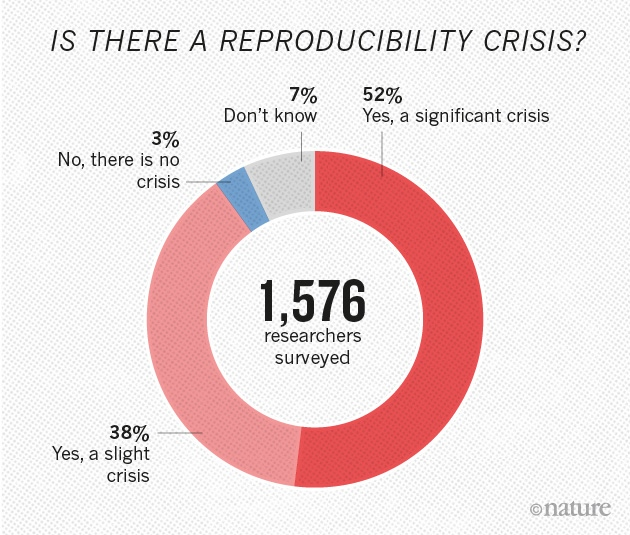
\includegraphics[width=0.6\textwidth,height=\textheight]{source/figures/nature_survey.jpeg}
\caption{Resultados de una encuesta sobre reproducibilidad.
baker500ScientistsLift2016}
\end{figure}

A día de hoy, los estudios suelen ofrecer los resultados en forma de
gráficas y tablas, pero en muchos casos carecen de la información
necesaria para poder contrastar los resultados. Está información suele
ser, el entorno de ejecución, los datos originales y la implementación
de los propios métodos (modelos, algoritmos, etc) entre otros. Para
aumentar la accesibilidad de los estudios, los investigadores deben
asegurarse de ofrecer esta información además de las gráficas y tablas.

La verificación independiente tiene como objetivo la confirmación de
credibilidad y la extensión del conocimiento en un area. La
investigación relativa al Machine Learning o a otras areas donde se haga
uso del mismo, no está exenta de este requisito de la investigación
científica. Por tanto, adoptando un flujo de trabajo reproducible,
estamos ofreciendo a la audiencia las herramientas necesarias que
demuestran las decisiones tomadas y que permiten validar nuestros
resultados. Por otro lado, para que un estudio computacional pueda ser
reproducido correctamente por un investigador independiente es necesario
el acceso completo a los datos, código, parámetros de los experimentos,
información sobre el entorno de ejecución, etc.

Otro motivo de interés para la búsqueda de la reproducibilidad es el de
facilitar el uso de nuestros métodos por el resto de la comunidad
científica o incluso en aplicaciones comerciales. Ofreciendo acceso a
los datos y al código, como se ha comentado antes, permitimos que
nuestros métodos se puedan aplicar a otros problemas, tanto en
investigación como para fines comerciales, así como facilita la
extensión de nuestro trabajo.

En los últimos años nos hemos encontrado con muchos casos de
publicaciones científicas que muestran resultados difíciles o incluso
imposibles de reproducir. Este fenómeno se conoce como la crisis de la
reproducibilidad, donde incluso estudios prominentes no se pueden
reproducir. Este fenómeno ha estudiado de manera extensiva en otros
campos, pero en el area del Machine Learning está tomando últimamente
mucho importancia. Esto es debido a que tradicionalmente, los
experimentos científicos se deben describir de tal forma que cualquiera
pueda replicarlos, sin embargo, los experimentos computacionales tienes
varias complicaciones que los hacen particularmente difíciles de
replicar: versiones de software, dependencias concretas, variaciones del
hardware, etc.

Con motivo de esta crisis de la reproducibilidad que afecta en gran
medida a AI/ML, conferencias como NeurIPS han optado por añadir este
factor en su proceso de revisión, e implementan políticas para alentar
el código compartido. Por otro lado, algunos autores (incluido nosotros)
han propuesto herramientas para facilitar la reproducibilidad, mientras
que otros han propuesto una serie de reglas o heurísticas que para
evaluar este aspecto.

\hypertarget{tipos-de-reproducibilidad}{%
\subsection{Tipos de reproducibilidad}\label{tipos-de-reproducibilidad}}

Para poder atajar de una manera directa y eficiente el problema de la
reproducibilidad es necesario separarla en diferentes niveles. Esta
separación nos permite desarrollar una serie de buenas prácticas y
herramientas específicas para cada nivel, así como ver de una manera
clara que aspectos se pueden recoger en un framework común, y cuales son
inherentes del estudio científico en cuestión. Entre los niveles de
reproducibilidad podemos destacar:

\begin{itemize}
\item
  Reproducibilidad computacional: Cuando se provee con información
  detallada del código, software, hardware y decisiones de
  implementación.
\item
  Reproducibilidad empírica: Cuando se provee información sobre
  experimentación empírica no computacional u observaciones.
\item
  Reproducibilidad estadística: Cuando se provee información sobre la
  elección de los test estadísticos, umbrales, p-valores, etc.
\end{itemize}

Una vez hecha separación del problema en tres capas, podemos ver
claramente que la reproducibilidad computacional debe ser nuestro
objetivo a la hora de desarrollar el framework. Mientras que la
reproducibilidad empírica se puede conseguir en mayor medida, haciendo
los datos accesibles, la reproducibilidad estadística se consigue
mediante el desarrollo de un diseño inicial del estudio. En este diseño
se especifica la hipótesis base, las asunciones del problema, los test
estadísticos a realizar, y los p-valores correspondientes. El establecer
las bases estadísticas sobre las que se va a desarrollar el estudio de
antemano, nos puede ayudar además a evitar problemas como el p-hacking.

Por otro lado, el término reproducibilidad además de poder descomponerse
según la información o parte del trabajo que se esté tratando,
llamémosla la escala o eje horizontal, también se puede descomponer en
otro eje, llamémosle vertical, que indica como de replicable y
reproducible es un estudio en su conjunto. Los niveles de esta nueva
escala son los siguientes:

\begin{itemize}
\item
  \textbf{Investigación revisable}. Las descripciones de los métodos de
  investigación pueden ser evaluados de manera independiente y los
  resultados juzgados. Esto incluye tanto los tradicionales peer-review,
  community-review, y no implica necesariamente reproducibilidad.
\item
  \textbf{Investigación replicable}. Se ponen a disposición del publico
  las herramientas que necesarias para replicar los resultados, por
  ejemplo se ofrece el el código de los autores para producir las
  gráficas que se muestran en la publicación. En este caso, las
  herramientas pueden tener un alcance limitado, ofreciendo los datos ya
  procesados y esenciales, así como ofreciéndolas mediante petición
  exclusivamente.
\item
  \textbf{Investigación confirmable}. Las conclusiones del estudio se
  pueden obtener sin el uso del software proporcionado por el autor.
  Pero se debe ofrecer una completa descripción de los algoritmos y la
  metodología usados en la publicación y cualquier material
  complementario necesario.
\item
  \textbf{Investigación auditable}. Cuando se registra la suficiente
  información sobre el estudio (incluidos datos y programas
  informáticos) para que la investigación pueda ser defendida
  posteriormente si es necesario o para llevar a cabo una resolución en
  caso de existir diferencias entre confirmaciones independientes. Esta
  información puede ser privada, como con los tradicionales cuadernos de
  laboratorio.
\item
  \textbf{Investigación abierta o reproducible}. Investigación auditable
  disponible abiertamente. El código y los datos se encuentran lo
  suficientemente bien documentados y accesibles al publico para que la
  parte computacional se pueda auditar, y lo resultados del estudio se
  puedan replicar y reproducir de manera independiente. También debe
  permitir extender los resultados o aplicar el método desarrollado a
  nuevos problemas.
\end{itemize}

\hypertarget{aspectos-cruxedticos}{%
\subsection{Aspectos críticos}\label{aspectos-cruxedticos}}

Una vez hemos definido los diferentes niveles de reproducibilidad, vamos
a definir los aspectos que consideramos críticos para lograr una
investigación \emph{abierta o reproducible}.

\begin{itemize}
\item
  \textbf{Conjunto de datos}: La información sobre la localización y el
  proceso de extracción de los datos. Este factor es determinante a la
  hora de hacer un estudio reproducible. El objetivo es el de facilitar
  los datos y/o la forma de extraerlos. En caso de que los datos no sean
  accesibles públicamente, o que los datos que se ofrezcan no sean los
  extraídos en crudo, estaríamos ante un \emph{estudio replicable}, pero
  no reproducible.
\item
  \textbf{Preprocesado de datos}: En este aspecto se recogen los
  diferentes pasos del proceso de transformación de los datos. Un
  investigador independiente debería ser capaz de repetir los datos de
  preprocesado fácilmente. Sería también interesante incluir datos ya
  preprocesados con los que comparar y validar que las transformaciones
  se han realizado correctamente. Estos procedimientos no son sencillos
  de documentar ni de compartir. En algunas ocasiones, las
  transformaciones se realizan en software privativos o utilizando una
  interfaz gráfica. En esos casos, en lugar de ofrecer los scripts de
  preprocesado, sería más interesante dar una descripción detallada de
  como los datos se han transformado. Además, sugerimos favorecer las
  herramientas de código libre en caso de que existan como alternativa a
  algunas de las herramientas privadas.
\item
  \textbf{Partición de los datos}: En caso de que los datos se separen,
  por ejemplo para ajustar un modelo y validarlo, es necesario
  proporcionar los detalles de como se ha realizado esta separación. En
  el caso de que dicha separación sea aleatoria, como mínimo se debe
  proporcionar la semilla y el tipo de muestreo (estratificado o no, por
  ejemplo). Aunque preferiblemente, todo este procedimiento debe estar
  recogido en un script.
\item
  \textbf{Ajuste del modelo}: Corresponde a toda la información relativa
  al ajuste de un modelo. En este caso, es necesario hacer disponible
  toda la información posible en relación a este proceso y a las
  decisiones tomadas. La información mínima que se debe proporcionar es:

  \begin{enumerate}
  \def\labelenumi{\arabic{enumi}.}
  \tightlist
  \item
    Parámetros del experimento
  \item
    Métodos propuestos: detalles de implementación, algoritmos, código,
    etc (si es aplicable).
  \end{enumerate}
\item
  \textbf{Evaluación del modelo}: Información sobre como se evalúa un
  modelo entrenado. Información similar al punto anterior se aplica
  aquí.
\item
  \textbf{Control de la estocásticidad}: La mayoría de operaciones en
  Machine Learning tienen un factor de aleatoriedad. Por tanto, es
  esencial establecer los valores de las semilla que controlar dichos
  procesos. La mayoría de herramientas de cálculo científico ofrecen
  algún método para establecer la semilla del generador de números
  aleatorios.
\item
  \textbf{Entorno software}: Debido al hecho de que los paquetes/módulos
  de software están en continuo desarrollo y sufren posibles
  alteraciones de los algoritmos internos, es importante que los
  detalles del entorno de software utilizado: módulos, paquetes y
  números de versión\ldots, estén disponible.
\item
  \textbf{Entorno hardware}: Algunos estudios, sobre todo los que
  contienen grandes cantidades de datos, son reproducibles
  exclusivamente cuando se ejecutan en una cierta máquina, o al menos,
  cuando se cumplen unos requisitos de hardware determinados. Otro
  problema que surge en algunos casos y que está estrechamente
  relacionado con el punto anterior, es el de las versiones de los
  drivers. Por este motivo, se requiere una correcta documentación de
  los recursos utilizados, tanto GPU como CPU, así como de las versiones
  de sus drivers correspondientes.
\end{itemize}

\hypertarget{proceso-de-ciencia-de-datos-y-deuda-tuxe9cnica}{%
\section{Proceso de ciencia de datos y deuda
técnica}\label{proceso-de-ciencia-de-datos-y-deuda-tuxe9cnica}}

La mayoría de proyectos de ciencia de datos recogen una serie de pasos
distinguidos. Una vez definido el caso comercial (el producto), y la
métrica que mide el éxito, los pasos para llevar a cabo un proyecto de
Machine Learning son los siguientes:

\begin{itemize}
\item
  \textbf{Extracción de datos}: Se seleccionan e integran datos de
  diferentes fuentes que sean relevantes para el problema.
\item
  \textbf{Análisis de datos}: En este paso se realiza un análisis
  exploratorio (EDA) con el fin de comprender el modelo de datos,
  realizar asunciones, identificar posibles características relevantes,
  y preparar un plan para la ingeniería de características y el
  preprocesado de datos.
\item
  \textbf{Preparación de los datos}: Se preparan los datos para la tarea
  en cuestión. Se realizan las particiones de datos, se limpian y
  transforman los mismos para adaptarlos al problema, y se lleva a cabo
  la ingeniería de características. El resultado de este proceso es una
  seria de conjuntos de datos listos para entrenar, evaluar y validar
  modelos.
\item
  \textbf{Ajuste de modelos}: Aquí se lleva a cabo el entrenamiento de
  modelos. Se implementan diferentes algoritmos y se realiza un ajuste
  de hiperparámetros con el fin de obtener el mejor modelo posible.
\item
  \textbf{Evaluación de modelos}: Se evalúa el modelo utilizando los
  conjuntos de validación y/o test.
\item
  \textbf{Validación de modelos}: Se realiza una confirmación del
  rendimiento del modelo para comprobar que es adecuado para la
  implementación. Para ello se compara su rendimiento predictivo con un
  modelo de referencia determinado, denominado \textbf{baseline}.
\item
  \textbf{Entrega o despliegue del modelo}: Se implementa el modelo
  final en el \emph{entorno de destino} para hacer las predicciones
  disponibles a los usuarios.
\item
  \textbf{Monitorización del modelo}: Se supervisa el rendimiento del
  modelo con el fin de planificar las siguientes iteraciones.
\end{itemize}

\hypertarget{deuda-tuxe9cnica}{%
\subsection{Deuda técnica}\label{deuda-tuxe9cnica}}

Como se puede observar, los pasos de este proceso siguen un orden
estricto, lo cual lo hace resonar a un modelo de desarrollo en cascada.
Al igual que el resto de aplicaciones del desarrollo software, la deuda
técnica es un factor vital a tener en cuenta. Un factor que puede
ralentizar enormemente las iteraciones, y que se va acumulando en cada
paso del proceso. Además, la alta dependencia que hay en el orden de los
pasos del proceso de ciencia de datos, hace muy difícil la
refactorización.

La deuda técnica es un concepto acuñado en el desarrollo software para
describir aquellas decisiones, que se toman por falta de tiempo o
conocimiento, que provocan un coste adicional sobre los nuevos cambios
conforme pasan el tiempo. Este término está basado en el concepto de
\emph{deuda monetaria}, y al igual que este tipo de deuda, si no se paga
temprano, el coste adicional aumenta de manera exponencial
(\emph{intereses compuestos}). Algunas de las causas de deuda técnica
son: falta de tests, falta de documentación, falta de conocimiento,
presión comercial (deadlines irreales), refactorización tardía, etc.

Además de la deuda técnica originada por el propio desarrollo software,
existe unos elementos particulares al proceso de ciencia de datos que
pueden aumentar drásticamente esta deuda:

\begin{itemize}
\item
  \textbf{Bucles de retroalimentación}: Este problema ocurre cuando, de
  manera indirecta, la salida del modelo influencia la entrada al mismo.
  De esta forma, los sistemas de ML modifican su propio comportamiento
  conforme pasa el tiempo. Este tipo de errores parecen sencillos de
  resolver, pero en la práctica, conforme se integran diferentes
  sistemas la probabilidad de que estos se retroalimenten entre si es
  muy alta. Incluso si dos sistemas de ML parecen no estar relacionados,
  este problema puede surgir. Imagínese dos sistemas que predicen del
  valor de acciones de un mismo mercado para dos compañías distintas.
  Mejoras o peor aún bugs, de un sistema, pueden influir en el
  comportamiento del otro sistema.
\item
  \textbf{Cascadas de corrección}: Este problema ocurre cuando el modelo
  de ML no aprende lo que se esperaba, y se terminan aplicando una serie
  de parches (heurísticas, filtros, calibraciones, etc) sobre la salida
  del modelo. Añadir un parche de este tipo puede sen tentador incluso
  cuando no hay restricciones de tiempo. El problema principal es que la
  métrica que el modelo intenta optimizar se descorrelaciona con la
  métrica general del sistema. Conforme esta capa de heurísticas se
  vuelve más grande, es difícil reconocer cambios sobre el modelo de ML
  que mejoraren la métrica final, dificultando de esta forma la
  iteración y mejora continua.
\item
  \textbf{Características basura}: Características que no aportan nada
  al sistema, incluso pueden perjudicar el rendimiento. Algunas de las
  características basura que podemos encontrar son:

  \begin{itemize}
  \tightlist
  \item
    Características agrupadas: Cuando se agrupan varias características
    y se evalúan en conjunto, es difícil saber si todas las
    características aportan, o si simplemente hay algunas que son
    beneficiosas y otras no.
  \item
    ε-Características: Algunas características que se añaden mejoran muy
    poco el rendimiento del modelo. Aunque es tentador añadir este tipo
    de características, el problema emerge cuando dichas características
    dejan de mejorar el modelo o incluso lo empeoran cuando los datos
    cambian mínimamente.
  \item
    Características obsoletas: Conforme pasa el tiempo, algunas
    características se vuelven obsoletas, porque o bien no aportan la
    información correcta, o bien la información que aportan ya se recoge
    en otras variables. Para evitar este problema, revaluar la
    importancia de las características con el paso del tiempo.
  \end{itemize}
\item
  \textbf{Deuda de configuración}: Sistemas de ML están compuestos por
  diferentes partes, cada una con un configuración específica. Los
  modelos y pipelines en general, deben de ser fácilmente configurables.
  Además, la organización de ficheros y el sistema de configuración debe
  facilitar lo siguiente:

  \begin{itemize}
  \tightlist
  \item
    Modificar configuraciones existentes fácilmente
  \item
    Comparar y ver claramente la diferencias entre configuraciones de
    modelos
  \item
    Detectar configuraciones redundantes
  \item
    Revisión de código sobre las configuración y su inclusión en un
    control de versiones.
  \end{itemize}
\item
  \textbf{Deuda de reproducibilidad}: Como se verá en la sección
  siguiente, es importante que como investigadores, podemos reproducir
  experimentos y obtener los mismos resultados fácilmente. Aunque en los
  sistemas ML reales es realmente difícil conseguirlo; debido
  principalmente a la naturaleza no determinística de los algoritmos,
  del entrenamiento en paralelo, y de las interacciones con el mundo
  exterior.
\end{itemize}

\hypertarget{anti-patrones}{%
\subsection{Anti-patrones}\label{anti-patrones}}

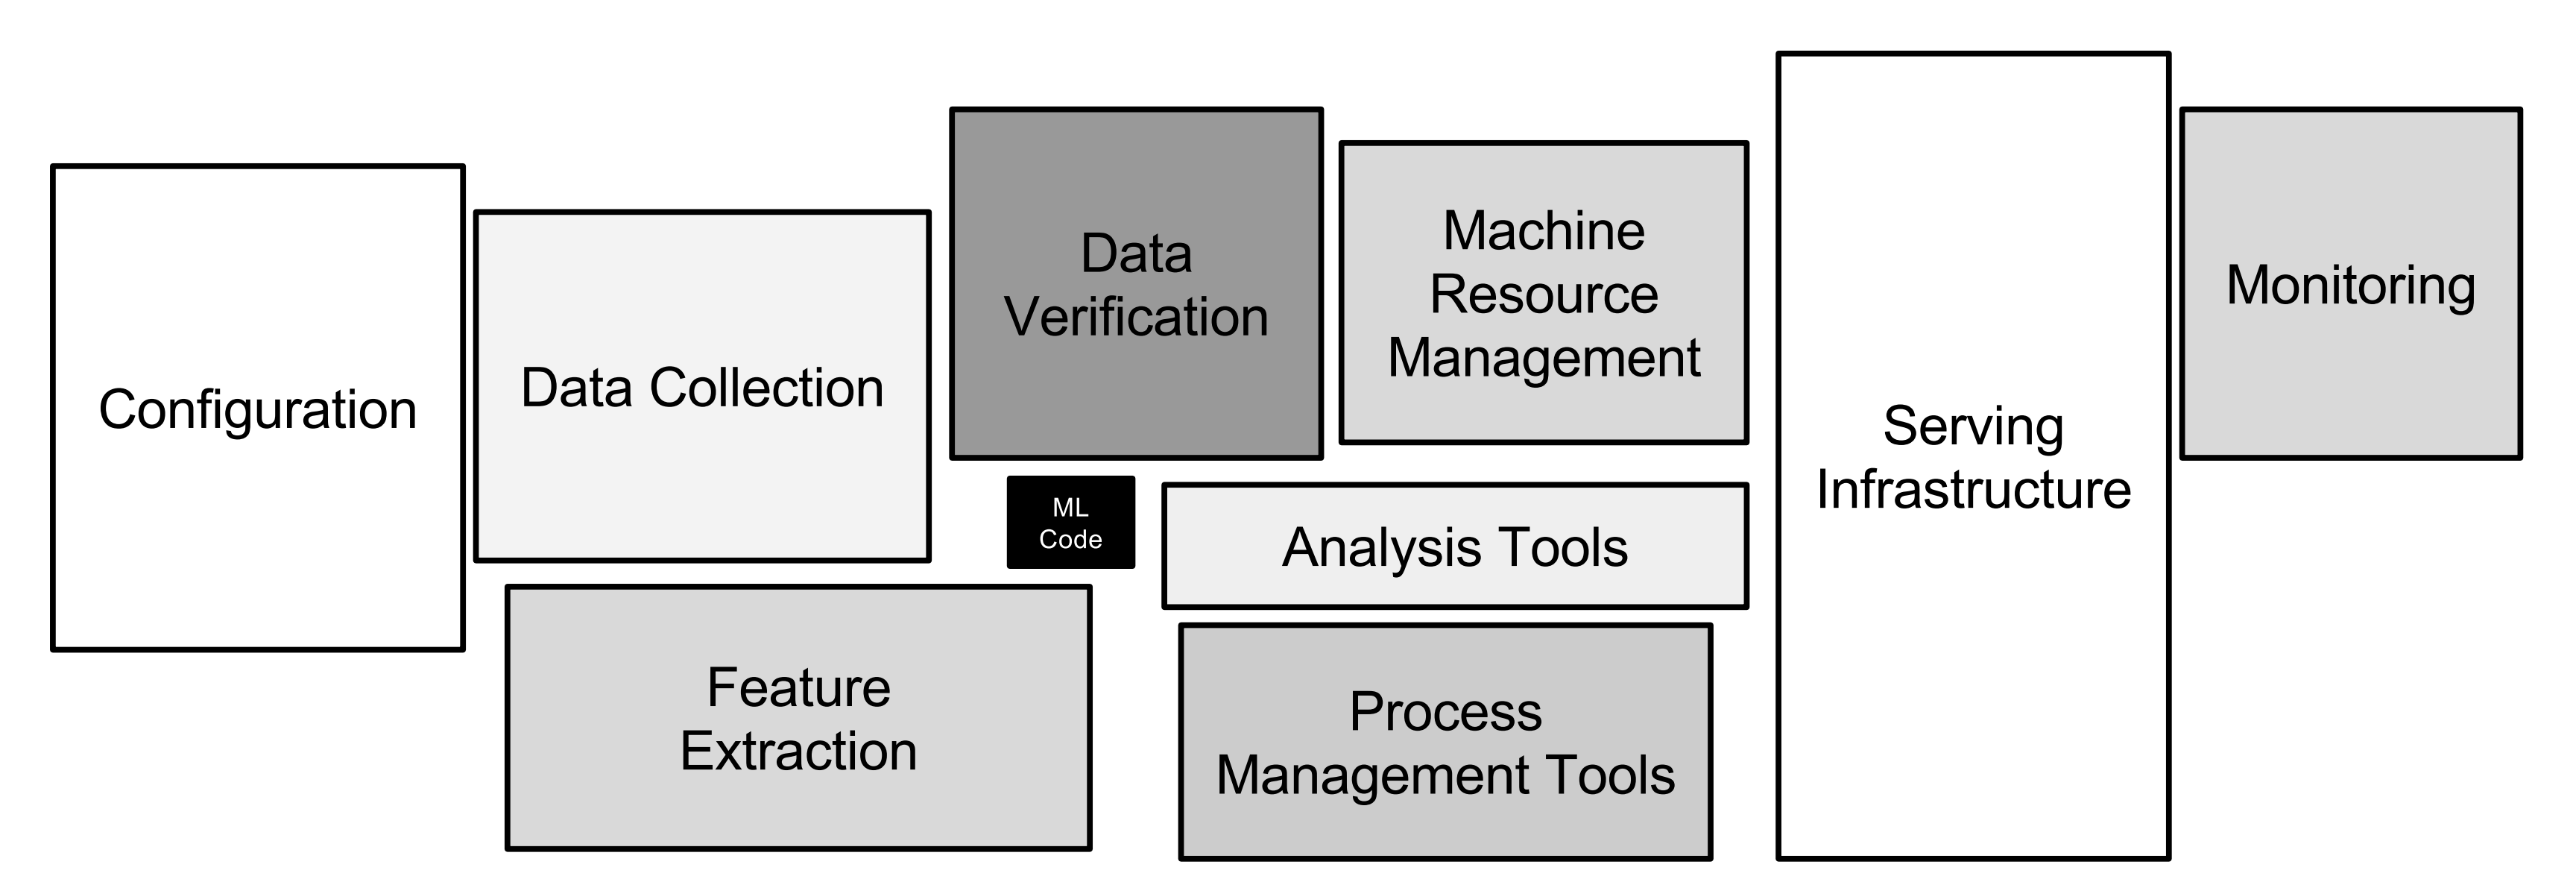
\includegraphics{source/figures/technical_debt.png}

Sorprendentemente, en la mayoría de sistemas de ML, solamente una
pequeña fracción del código está dedicado al entrenamiento y predicción.
El resto de código, conocido como \emph{plumbing}, es susceptible a una
serie de anti-patrones que se describen a continuación:

\begin{itemize}
\item
  \textbf{Código pegamento}: A pesar de que en la comunidad existen
  numerosos paquetes y soluciones para ML. El utilizar herramientas
  genéricas puede hacer que el sistema dependa mayoritariamente de
  ellas. Eso provoca que en algunos casos haya una gran cantidad de
  código solamente para introducir y extraer datos de estas soluciones
  \emph{open source}. Si nuestro sistema tienen una gran proporción del
  código dedicado a adaptar los datos, algoritmos, etc, a un paquete de
  propósito general, deberíamos plantearnos crear una solución propia.
\item
  \textbf{Junglas de pipelines}: La mayoría de sistema integran
  multiples fuentes de información. Estas fuentes de información, así
  como las transformaciones pertinentes sobre los datos, suelen
  evolucionar a lo largo del desarrollo. Esto induce a un caso
  particular de \emph{código pegamento} donde se hace muy complicado
  poder testear, recuperarse de errores, etc. Una forma de subsanar este
  problema, es diseñado el sistema holísticamente (teniendo en cuenta
  todo el pipeline), en lugar de enfocarse en los pasos intermedios.
  Además, también sería beneficioso, en la medida de lo posible, aplicar
  los conceptos de \emph{programación funcional}.
\item
  \textbf{Código muerto}: Los proyectos de ML se basan en la
  experimentación. Al cabo del tiempo, estos sistemas pueden acabar con
  una gran cantidad de código dedicados experimentos que nunca han visto
  la luz.
\item
  \textbf{Deuda de abstracción}: Los problemas anteriores reflejan una
  falta de abstracción para los sistemas de ML, como puede ser un
  lenguaje común de alto nivel para definir las fuentes de datos, modelo
  y predicciones.
\item
  \textbf{Code-smells más comunes}: Algunos de los indicadores de
  \emph{peligro} en la implementación de sistemas de ML son los
  siguientes:

  \begin{itemize}
  \tightlist
  \item
    \emph{Tipos de datos planos}: En un sistema robusto, la información
    producida en el mismo se almacena enriquecida. Se debe saber si un
    parámetro de un modelo es un threshold o no, si uen variable esta en
    escala logarítmica, etc. Así como debe haber claras indicaciones de
    como se ha producido la información y como se debe ser consumida.
  \item
    \emph{Multiples lenguajes}: Es tentador utilizar diferentes
    lenguajes para un mismo sistema de ML cuando hay soluciones o
    sintaxis conveniente para cada componente. Sin embargo, esto limita
    la movilidad del capital humano, así como complica el testing.
  \item
    \emph{Prototipos}: Todo sistema de ML parte de un prototipo. Sin
    embargo, es necesario un código bien testeado y listo para
    producción en cualquier parte de estos sistemas. Aunque es
    complicado llevarlo a la práctica cuando existen unas restricciones
    de tiempo fuertes.
  \end{itemize}
\end{itemize}

\hypertarget{machine-learning-operations-mlops}{%
\section{Machine Learning Operations
(MLOps)}\label{machine-learning-operations-mlops}}

Durante los últimos años, el papel de la ciencia de datos y del Machine
Learning ha tomado gran relevancia en la industria. En la actualidad, la
ciencia de datos se utiliza para resolver problemas complejos, y ofrecer
una gran variedad de productos de datos: traductores automáticos,
sistemas de recomendación, sistemas de trading de alta frecuencia,
etc.\\
La ciencia de datos ha podido ser aplicada a una variedad muy amplia de
campos, ha aportado valor en cada uno de ellos, incluso haya
revolucionado algunas industrias. Para que esto haya sido posible, y
para que siga siendo posible, es necesario una gran cantidad de datos,
recursos de computación (CPU y GPU) accesibles, hardware optimizado para
cálculo científico, así como una activa comunidad de investigadores.

El hecho de que cada vez más industrias estén implementado sistemas de
ML como productos o parte de productos comerciales, hace indispensable
unos flujos de desarrollo orientados a la industria. La ciencia de datos
parte originalmente de la experimentación, no obstante, conforme los
sistemas de ML se integran con el resto de componentes de una
organización, es necesario aplicar las técnicas y buenas prácticas
conocidas en el desarrollo software, con el fin de ofrecer a los
usuarios sistemas predictivos con valor comercial y mínimo coste. Los
científicos de datos pueden implementar y entrenar modelos localmente,
sin conexión a internet incluso, pero el verdadero desafío consiste en
implementar un sistema ML integrado, y operarlo en producción de manera
continua.

Como se ha detallado en la sección anterior, y como se muestra en la
figura X, el ciclo de desarrollo de un producto de un sistema ML implica
diferentes fases. El código relacionado con la propia implementación y
entrenamiento de modelos es mínimo comparado con el resto de código
necesario para el desarrollo de estos sistemas. Además, debido a la
necesidad de grandes cantidades de datos y de recursos computaciones
amplios, estos sistemas deben incluir otros módulos relativos a la
infraestructura: manejos de recursos, monitorización, automatización,
etc.

\hypertarget{devops.-definiciuxf3n}{%
\subsection{DevOps. Definición}\label{devops.-definiciuxf3n}}

Para poder desarrollar sistemas software complejos, la tendencia actual
es utilizar las técnicas de \emph{DevOps}. \emph{DevOps} es un conjunto
de prácticas en el desarrollo y operacionalización. Estas prácticas
aumentan la velocidad de implementación, reducen los ciclos de
desarrollo, y facilitan la entrega de actualizaciones. Entre las
prácticas recogidas en este concepto se incluyen:

\begin{itemize}
\item
  \textbf{Integración continua (CI)}: Esta práctica de desarrollo
  software permite a los desarrolladores ejecutar versiones y pruebas
  automáticas cuando se combinan cambios de código en el repositorio del
  proyecto. Esto permite validar y corregir errores con mayor rapidez,
  mejorando así la calidad del software.
\item
  \textbf{Entrega continua (CD)}: Esta práctica de desarrollo software
  se basa en la compilación, prueba y preparación automática de
  artefactos. Estos artefactos se generan automáticamente cuando se
  producen cambios en el código y se entregan a la fase de producción.
  De esta forma, las actualizaciones a los usuarios finales se entregar
  con mínimo esfuerzo. Travis o CircleCI son algunos de los servicios
  que ofrecen tanto \emph{Integración Continua} como \emph{Entrega
  Continua}.
\item
  \textbf{Microservicios}: La arquitectura de microservicios es un
  enfoque de diseño que permite crear una aplicación a partir de un
  conjunto de servicios pequeños. Cada servicio se ejecuta de manera
  independiente y se comunica con los otros servicios a través una
  interfaz ligera, normalmente HTTP. Recientemente, algunos otros
  protocolos de nivel superior como GRPC o GraphQL se están utilizando
  para la interconexión de estos servicios.
\item
  \textbf{Infraestructura como código}: Aprovisionar y administrar
  infraestructura con técnicas de desarrollo de programación y
  desarrollo software, como el control de versiones. Algunos servicios
  como AWS, CloudFormation o Terraform permiten aprovisionar y gestionar
  infraestructuras utilizando lenguajes de programación o ficheros de
  configuración.
\item
  \textbf{Monitorización y registro}: Monitorizar métricas y registros
  para analizar el desempeño de las aplicaciones y la infraestructura
  sobre la experiencia usuario.
\item
  \textbf{Comunicación y colaboración}: Uno de los aspectos claves en la
  filosofía \emph{DevOps} es el incremento de la comunicación y la
  colaboración en las organizaciones.
\end{itemize}

\hypertarget{devops-aplicado-al-machine-learning}{%
\subsection{DevOps aplicado al Machine
Learning}\label{devops-aplicado-al-machine-learning}}

\emph{MLOps} se fundamenta en los principios y prácticas de
\emph{DevOps}. Nociones, como se ha comentado previamente, orientadas a
la eficiencia en el desarrollo: integración y entrega continuos,
monitorización, etc. \emph{MLOps} aplica estos principios para la
entrega de sistemas de ML a escala, resultando en:

\begin{itemize}
\tightlist
\item
  Tiempo de comercialización de soluciones basadas en ML menor.
\item
  Ratio de experimentación mayor que fomenta la innovación.
\item
  Garantía de calidad, confidencialidad y \emph{IA ética}.
\end{itemize}

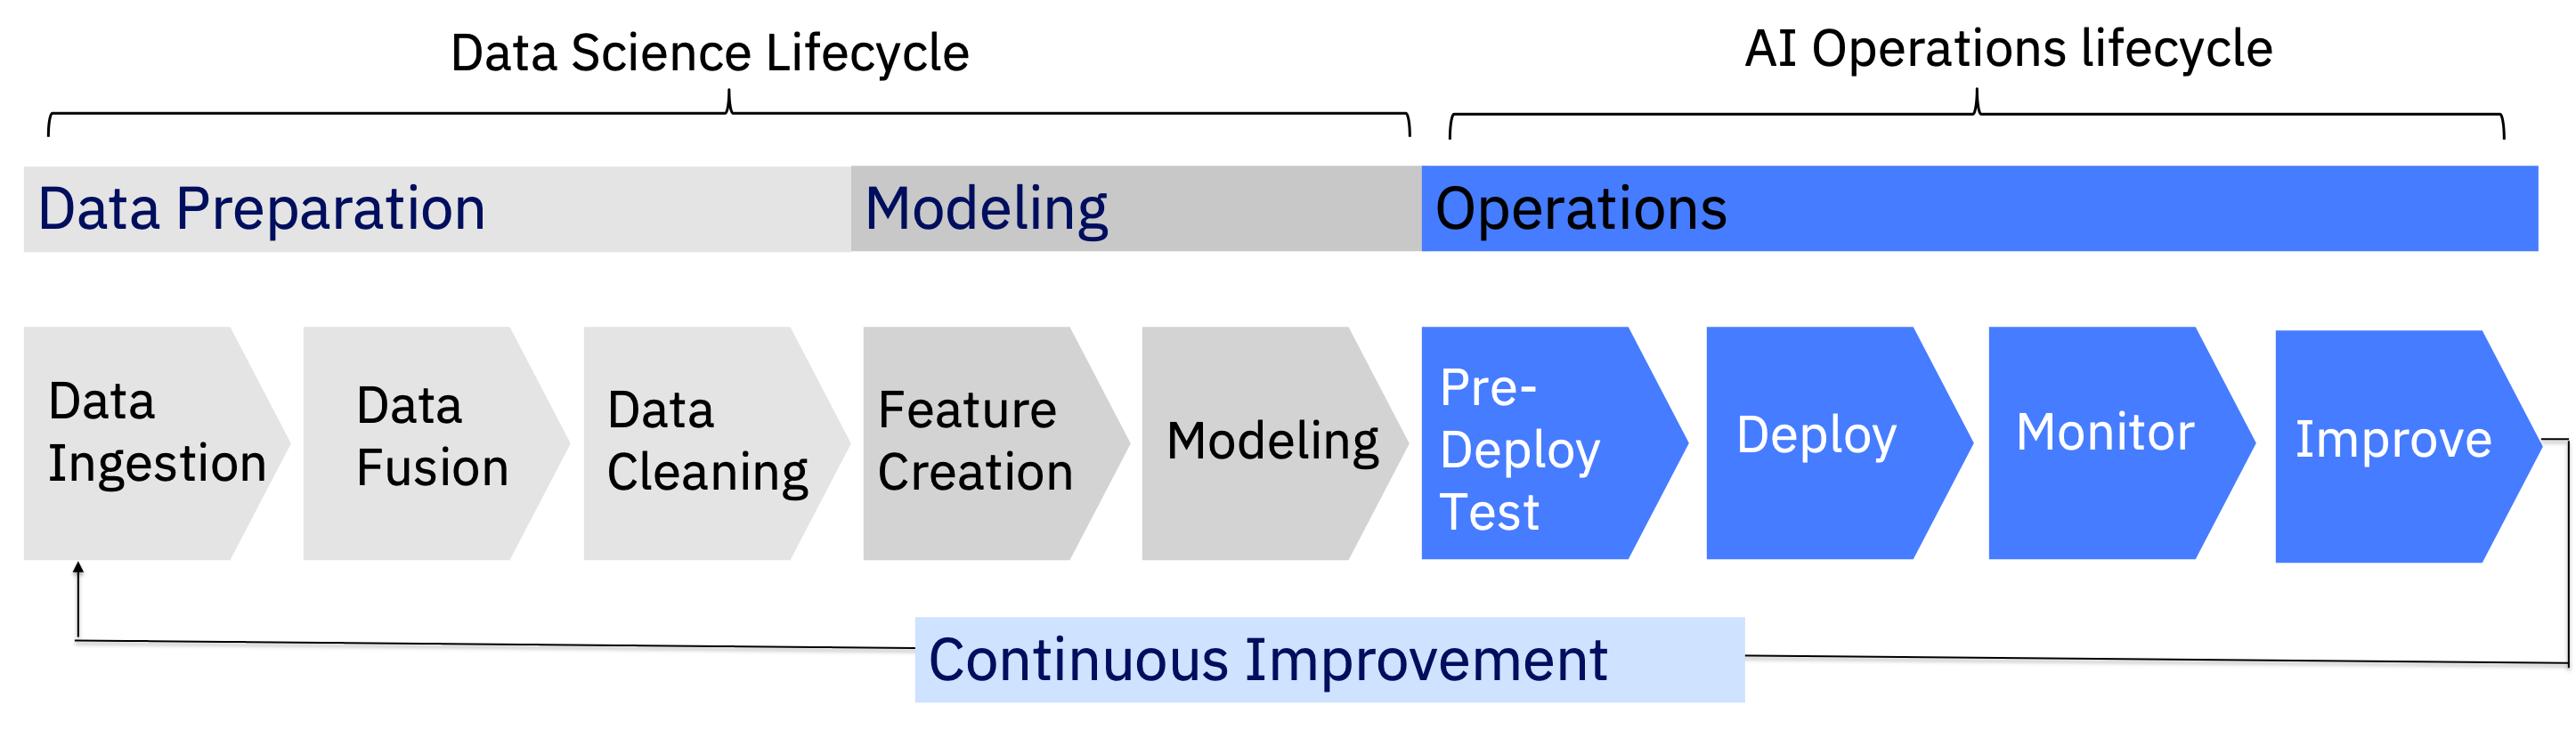
\includegraphics{source/figures/mlops_overview.png}

Para poder analizar la interacción entre DevOps y el desarrollo de
sistemas de ML, es necesario destacar las tareas claves de este proceso.
Teniendo en cuenta el proceso de ciencia de datos descrito en la sección
anterior, (también representado en la Figura X) podemos destacar las
siguientes tareas:

\begin{itemize}
\item
  \textbf{Recolectar y preparar datos}: Generar y preparar los conjuntos
  de datos para el entrenamiento.
\item
  \textbf{Aprovisionar y gestionar la arquitectura}: Establecer los
  entornos de computación donde se se entrenan los modelos y despliegan
  los modelos.
\item
  \textbf{Entrenar modelos}: Desarrollar el código de entrenamiento y
  evaluación, y ejecutarlos en la infraestructura aprovisionada.
\item
  \textbf{Registrar de modelos}: Después de la ejecución de un
  experimento, el modelo resultado se almacena en el \emph{registro de
  modelos}.
\item
  \textbf{Desplegar el modelo}: Validar los resultados del modelo,
  desplegarlo en el \emph{entorno objetivo}.
\item
  \textbf{Operar el modelo}: Operar el modelo en producción
  monitorizándolo para conocer su rendimiento, detectar \emph{desfases
  de datos}, alerta de fallas, etc.
\end{itemize}

Esta secuencia de actividades se corresponde con un \emph{pipeline}. La
dificultad principal en el diseño de este pipeline es que cada paso es
altamente iteratable. Es decir, los modelos necesitar ser modificados,
los resultados testeados, se añaden nuevas fuentes de información, etc.
El poder iterar de una manera eficiente es fundamental para este tipo de
sistemas. Además, existen ciertos requisitos que solamente se conocen
una vez que el modelo se monitoriza. Como pueden ser el \emph{desfase de
datos}, sesgo inherente o fallas del sistema.

Para responder a estos desafíos de manera exitosa, los equipos de ML
deben implementar las siguientes prácticas.

\begin{itemize}
\item
  \textbf{Reproducibilidad}: Como se ha explicado en al principio del
  capítulo, este aspecto es fundamental y es uno de los objetivos de
  MLOps. Cuando se automatizan los diferentes pasos del proceso de
  ciencia de datos, es necesario que cada paso sea determinista, para
  evitar resultados indeseables.
\item
  \textbf{Reusabilidad}: Para poder ajustarse a los principios de
  \emph{entrega continua}, la \emph{pipeline} necesita empaquetar y
  entregar modelos y código de una manera consistente, tanto a los
  entornos locales de entrenamiento como a los \emph{entornos
  objetivos}, de forma que una misma configuración pueda arrojar los
  mismos resultados.
\item
  \textbf{Manejabilidad} -- La habilidad de aplicar regulación, rastrear
  los cambios en los modelos y código a lo largo del ciclo de vida, y
  permitir a los managers y gestores de equipo medir el progreso del
  proyecto y el valor comercial.
\item
  \textbf{Automatización} -- Al igual que en DevOps, para aplicar
  integración y entrega continua se require automatización. Los
  \emph{pipelines} deben ser fácilmente repetibles, especialmente cuando
  se aplica gobernanza, o testing. Desarrolladores y científicos de
  datos pueden adoptar MLOps para colaborar y asegurar que las
  iniciativas de ML están alineadas con el resto de entrega del
  software, así como con el negocio en general.
\end{itemize}

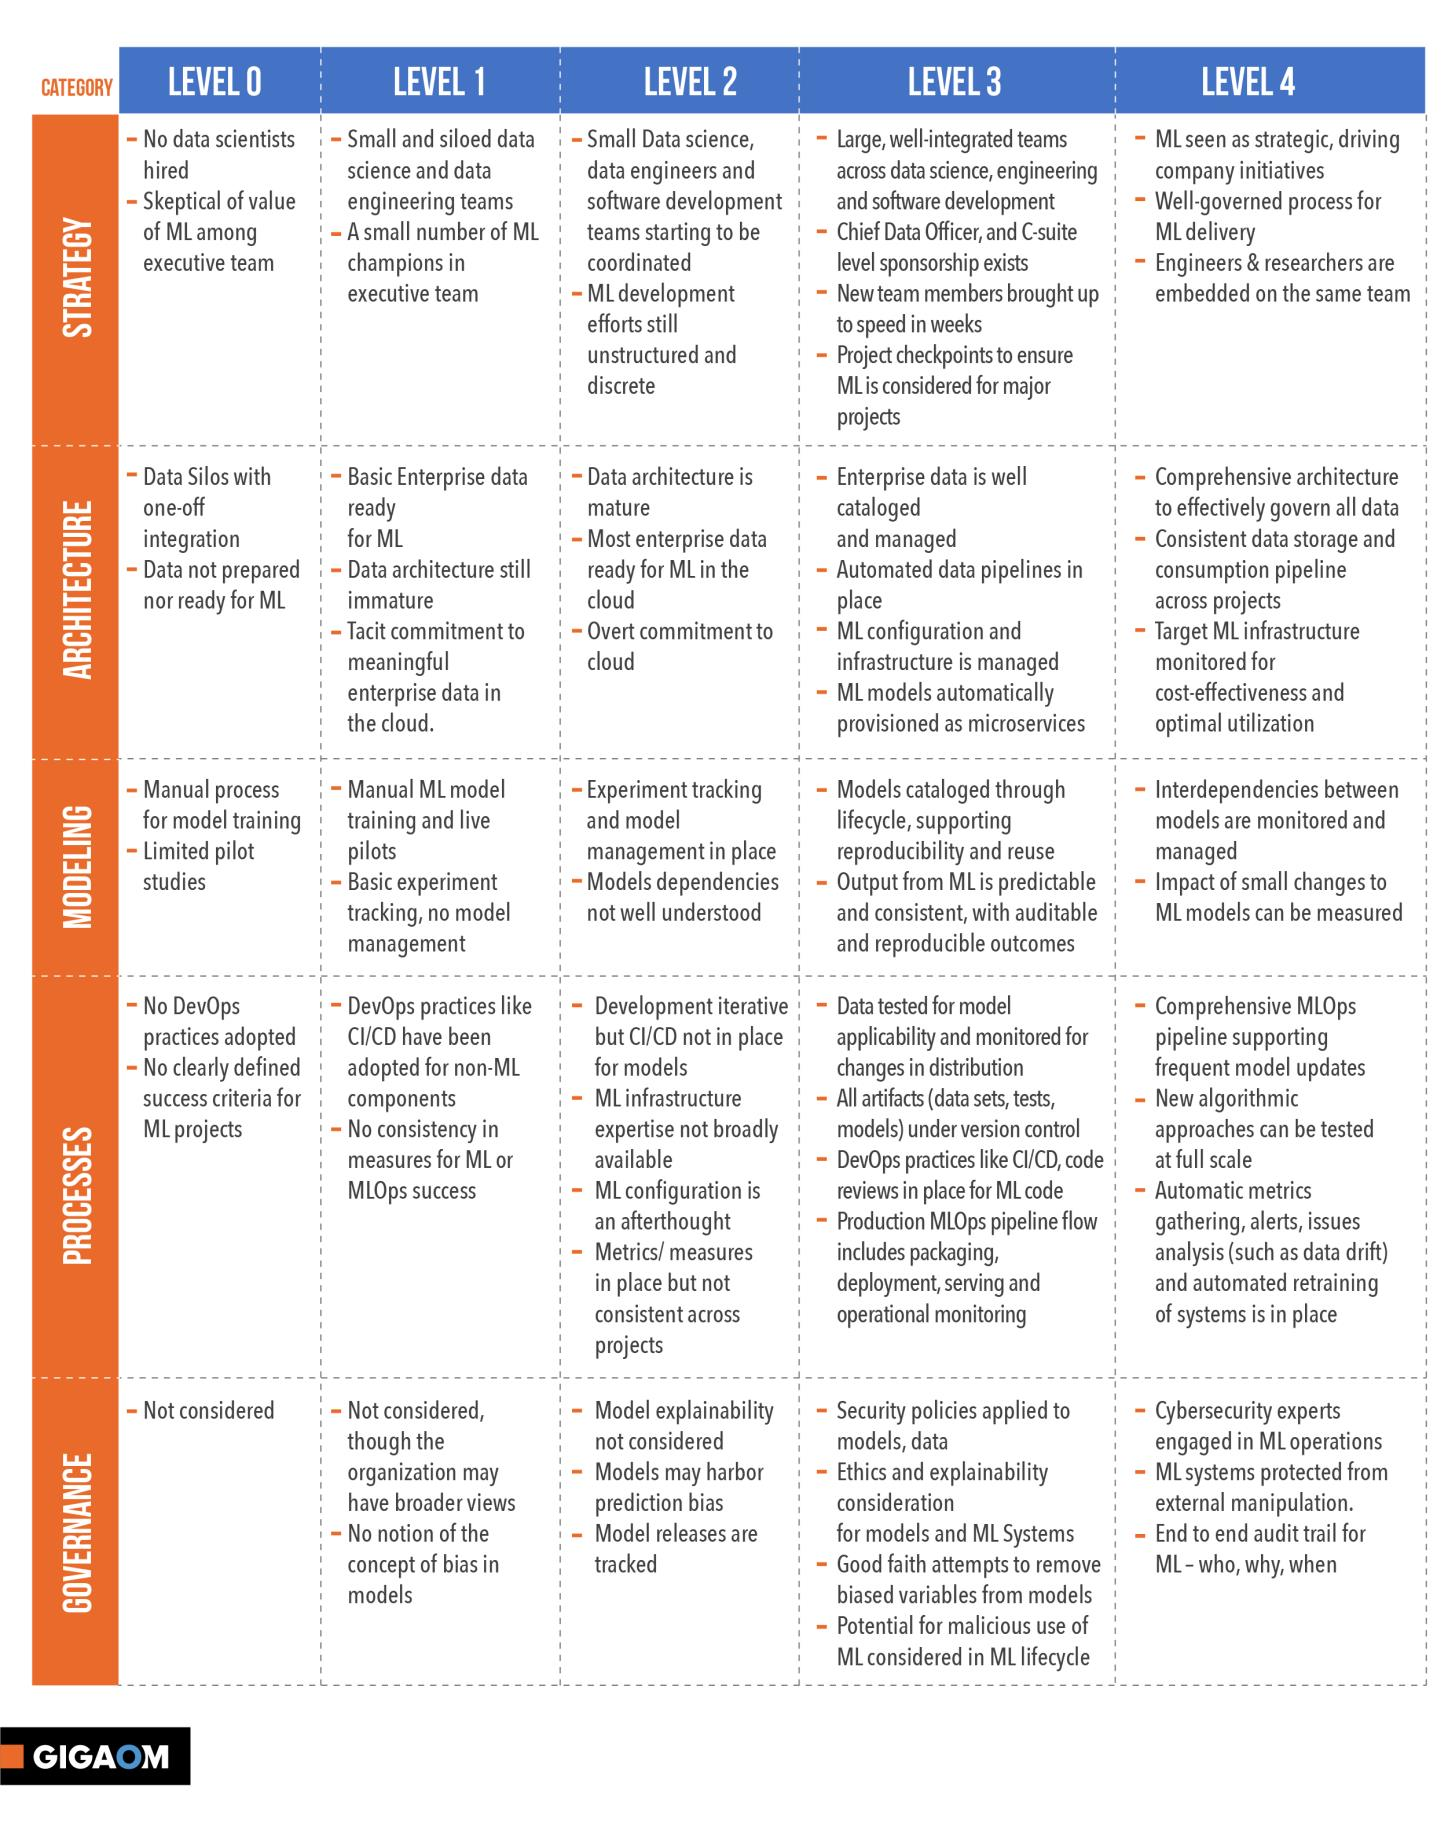
\includegraphics{source/figures/mlops_levels.jpg}

Las prácticas anteriores son un indicador de la madurez del equipo de
ciencia de datos, así como de las relaciones con el resto de equipos de
desarrollo, y la compañía. Cada compañía puede implementar estas
prácticas a diferentes niveles. El modelo de madurez de MLOps
\emph{MLOps Maturity Model}. En la figura X se muestra un resumen de
cada nivel según este modelo. Las categorías recogidas en él son las
siguientes:

\begin{itemize}
\tightlist
\item
  \textbf{Estrategia}: Como la compañía puede alinear las actividades de
  MLOps con las prioridades ejecutivas, de organización y culturales.
\item
  \textbf{Arquitectura} -- La habilidad para manejar datos, modelos,
  entornos de despliegue y otros artefactos de manera unificada.
\item
  \textbf{Modelado} -- Habilidades de ciencia de datos y experiencia,
  que sumados al conocimiento de dominio, permitan el desarrollo y
  entrega de sistema de ML para dicho dominio.
\item
  \textbf{Procesos} -- Entrega y despliegue de actividades de manera
  eficiente, efectiva y mensurable, que impliquen científicos,
  ingenieros y administradores.
\item
  \textbf{Gobernanza} -- En general, la habilidad para construir
  soluciones de inteligencia artificial seguras, responsables y justas.
\end{itemize}

\hypertarget{redes-neuronales}{%
\section{Redes neuronales}\label{redes-neuronales}}

Las redes neuronales son algoritmos de aprendizaje automático que han
adquirido una gran popularidad en los últimos años, y que han sido
desarrollados y utilizados en una gran variedad de problemas, desde
aprendizaje supervisado, hasta no supervisado, pasando por aprendizaje
por refuerzo y reducción de la dimensionalidad.

Para describir una red neuronal vamos a empezar por la arquitectura más
básica, una sola neurona. Una forma de representar dicha neurona en una
diagrama es la siguiente:

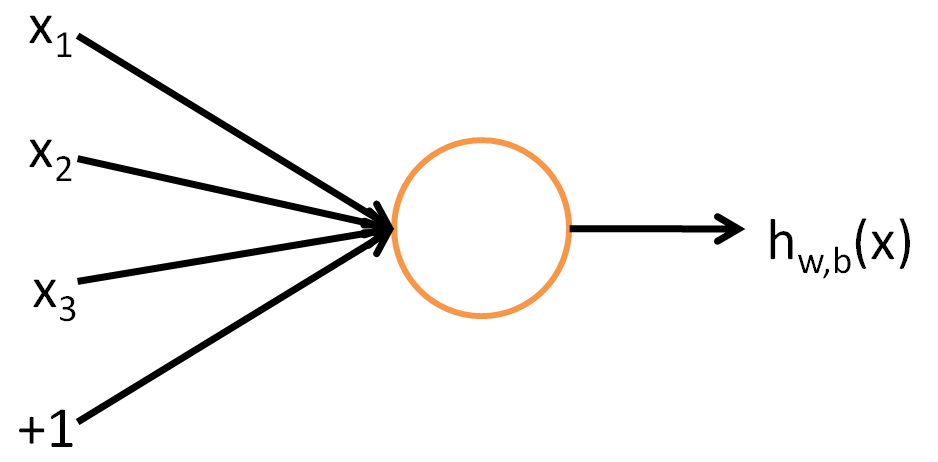
\includegraphics{source/figures/single_neuron.png}

Una neurona no es más que una unidad computacional que toma como entrada
un vector \(x\) (más un elemento a 1 para el sesgo), y cuya salida es
\(h_{W, b}(x)=f\left(W^{T} x\right)=f\left(\sum_{i=1}^{3} W_{i} x_{i}+b\right)\),
donde \(f: \mathbb{R} \mapsto \mathbb{R}\) es la llamada \textbf{función
de activación}. Entre las función de activación más comunes se
encuentran: sigmoide, tanh, RELU, LeakyRELU y Swish.

Una red neuronal se construye juntando varias neuronas, de forma que las
salidas de unas neuronas son las entradas de otra, como se muestra en la
figura X. En la figura, los círculos representan una neurona, y aquellos
con etiqueta +1 son las \textbf{unidades de sesgo}. Por otro lado, las
unidades o neuronas se agrupan en capas, una capa está representada como
una columna de círculos. Dentro de estas capas, podemos diferenciar tres
tipos: la capa de entrada (más a la izquierda), la capa interna, y la
capa de salida que solamente contiene una neurona (a la derecha).

Vamos a denotar, \(n_l\) como el numero de capas de nuestra red,
\(n_l=3\) en nuestro ejemplo. A la capa de entrada la denotamos como
\(L_1\), y la capa de salida por tanto sería \(L_{n_l}\). Nuestra red
neuronal tiene como parámetros
\((W, b)= \left(W^{(1)}, b^{(1)}, W^{(2)}, b^{(2)}\right)\), donde cada
elemento \(W_{i j}^{(l)}\) corresponde con el parámetro asociado a la
conexión entre la neurona \(j\) de la capa \(l\) y la neurona \(i\) de
la capa \(l + 1\). Por otro lado, \(b_{i}^{(l)}\) es el sesgo asociado a
la unidad \(i\) de la capa \(l + 1\).

Podemos denotar a la activación (valor de salida) de una neurona \(i\)
de la capa \(l\) como \(a_{i}^{(l)}\). En el caso de la capa de entrada
(\(l = 1\)), es obvio que \(a_{i}^{(1)}=x_{i}\). Gracias a la notación
vectorial, podemos definir el vector de activaciones de una capa como:

\[
\begin{aligned}
z^{(l+1)} &=W^{(l)} a^{(l)}+b^{(l)} \\
a^{(l+1)} &=f\left(z^{(l+1)}\right)
\end{aligned}
\]

Finalmente, la función hipótesis, o salida de la red, se puede definir
como:

\[h_{W, b}(x)=a^{(n_l)}=f\left(z^{(n_l)}\right)\]

Teniendo en cuenta esta nomenclatura, la función de salida de la red
mostrada en la figura X, corresponde con la siguiente ecuación:

\[
\begin{aligned}
z^{(2)} &=W^{(1)} x+b^{(1)} \\
a^{(2)} &=f\left(z^{(2)}\right) \\
z^{(3)} &=W^{(2)} a^{(2)}+b^{(2)} \\
h_{W, b}(x) &=a^{(3)}=f\left(z^{(3)}\right)
\end{aligned}
\]

Una de las ventajas principales de usar la notación vectorial es que a
la hora de implementarlo, podemos aprovechar bibliotecas y rutinas de
algebra lineal con implementaciones eficientes como BLAS o LAPACK.

\hypertarget{algoritmo-de-propagaciuxf3n-hacia-atruxe1s}{%
\subsection{Algoritmo de propagación hacia
atrás}\label{algoritmo-de-propagaciuxf3n-hacia-atruxe1s}}

Suponiendo que tenemos un conjunto de datos
\(\left\{\left(x^{(1)}, y^{(1)}\right), \ldots,\left(x^{(m)}, y^{(m)}\right)\right\}\)
con \(m\) ejemplos. Podemos entrenar una red neuronal usando gradiente
descendiente. La función de coste a optimizar para un ejemplo es la
siguiente:

\[J(W, b ; x, y)=\frac{1}{2}\left\|h_{W, b}(x)-y\right\|^{2}\]

Dado un conjunto de entrenamiento de \(m\) ejemplos, el coste total se
define como:

\[
\begin{aligned}
J(W, b) &=\left[\frac{1}{m} \sum_{i=1}^{m} J\left(W, b ; x^{(i)}, y^{(i)}\right)\right]+\frac{\lambda}{2} \sum_{l=1}^{n_{l}-1} \sum_{i=1}^{s_{l}} \sum_{j=1}^{s_{l+1}}\left(W_{j i}^{(l)}\right)^{2} \\
&=\left[\frac{1}{m} \sum_{i=1}^{m}\left(\frac{1}{2}\left\|h_{W, b}\left(x^{(i)}\right)-y^{(i)}\right\|^{2}\right)\right]+\frac{\lambda}{2} \sum_{l=1}^{n_{l}-1} \sum_{i=1}^{s_{l}} \sum_{j=1}^{s_{l+1}}\left(W_{j i}^{(l)}\right)^{2}
\end{aligned}
\]

El primer termino de \(J(W, b)\) es la media de los cuadrados de los
residuos (errores). El segundo termino corresponde con la
regularización. El término \(\lambda\) controla la importancia relativa
de la regularización. Esta función de coste se utiliza tanto para
regresión como para clasificación. En el caso de la clasificación, \(y\)
toma los valores 0 o 1 según la clase que corresponda. Si usamos
\(tanh\) como función de activación en la salida en lugar de la
sigmoide, usaríamos los valores -1 y 1 en su lugar.

El objetivo es minimizar \(J(W, b)\) como función de \(W\) y \(b\). Para
llevar a cabo esta optimización, debemos inicializar \(W\) y \(b\) con
valores aleatorios próximos a cero, por ejemplo, con valores muestreados
de \(\mathcal{N}\left(0, \epsilon^{2}\right)\). El motivo por el que es
importante inicializar aleatoriamente los pesos, es para \textbf{romper
la simetría}. Posteriormente, aplicamos un algoritmo de optimización,
como puede ser \emph{gradiente descendiente}. Una iteración de gradiente
descendiente actualizaría los pesos de la siguiente forma:

\[
\begin{aligned}
W_{i j}^{(l)} &:=W_{i j}^{(l)}-\alpha \frac{\partial}{\partial W_{i j}^{(l)}} J(W, b) \\
b_{i}^{(l)} &:=b_{i}^{(l)}-\alpha \frac{\partial}{\partial b_{i}^{(l)}} J(W, b)
\end{aligned}
\]

El parámetro \(\alpha\) corresponde al ratio de aprendizaje. El
algoritmo de propagación hacia atrás nos ofrece una forma eficiente de
calcular las derivadas parciales necesarias para actualizar los pesos
mediante gradiente descendiente. Para calcular las derivadas parciales,
es necesario formular dichas derivadas.

\[
\begin{aligned}
\frac{\partial}{\partial W_{i j}^{(l)}} J(W, b) &=\left[\frac{1}{m} \sum_{i=1}^{m} \frac{\partial}{\partial W_{i j}^{(l)}} J\left(W, b ; x^{(i)}, y^{(i)}\right)\right]+\lambda W_{i j}^{(l)} \\
\frac{\partial}{\partial b_{i}^{(l)}} J(W, b) &=\frac{1}{m} \sum_{i=1}^{m} \frac{\partial}{\partial b_{i}^{(l)}} J\left(W, b ; x^{(i)}, y^{(i)}\right)
\end{aligned}
\]

El motivo por el que ambas ecuaciones difieren, es que la regularización
no se aplica al sesgo. El algoritmo que nos permite calcular dichas
derivadas de manera eficiente es el siguiente:

\begin{enumerate}
\def\labelenumi{\arabic{enumi}.}
\tightlist
\item
  Una pasada hacia adelante computando los valores de todas las neuronas
  a partir de la segunda capa.
\item
  Para cada neurona \(i\) de la capa \(n_l\) de salida, calculamos:
  \[\delta_{i}^{\left(n_{l}\right)}=\frac{\partial}{\partial z_{i}^{\left(n_{l}\right)}} \frac{1}{2}\left\|y-h_{W, b}(x)\right\|^{2}=-\left(y_{i}-a_{i}^{\left(n_{l}\right)}\right) \cdot f^{\prime}\left(z_{i}^{\left(n_{l}\right)}\right)\]
\item
  Para cada capa \(l=n_{l}-1, n_{l}-2, n_{l}-3, \dots, 2\) y para cada
  neurona \(i\) en \(l\), calcular:
  \[\delta_{i}^{(l)}=\left(\sum_{j=1}^{s_{l+1}} W_{j i}^{(l)} \delta_{j}^{(l+1)}\right) f^{\prime}\left(z_{i}^{(l)}\right)\]
\item
  Finalmente, las derivadas parciales vienen dadas por: \[
   \begin{aligned}
   \frac{\partial}{\partial W_{i j}^{(l)}} J(W, b ; x, y) &=a_{j}^{(l)} \delta_{i}^{(l+1)} \\
   \frac{\partial}{\partial b_{i}^{(l)}} J(W, b ; x, y) &=\delta_{i}^{(l+1)}
   \end{aligned}
   \]
\end{enumerate}

\hypertarget{autoencoders}{%
\section{Autoencoders}\label{autoencoders}}

Autoencoders son redes neuronales entrenadas para reconstruir la
entrada, es decir, para copiar la entrada en la salida. Internamente,
estas arquitecturas contienen un capa interna llamada \textbf{código}.
Este código es una representación de los datos de entrada en un espacio
vectorial de dimensión igual o distinta a los mismo. La red puede
plantearse como la suma de dos partes bien diferenciadas: un codificador
(encoder), que representa una función \(h=f(x)\), y un decodificador
(decoder) que produce una reconstrucción de la salida \(r = g(h)\). Esta
arquitectura se puede ver fácilmente en la figura INSERTAR FIGURA.

Si diseñamos un autoencoder que únicamente se encargue de copiar la
entrada en la salida, es decir, si simplemente es capaz de mapear
\(g(f(x)) = x\) para todos los valores de \(x\), no es especialmente
útil. Sin embargo, podemos diseñar autoencoders que no se limiten a
copiar la información de entrada, sino que aprendan patrones de los
datos y los utilicen para la reconstrucción. Este es el objetivo de los
autoencoders. Cuando restringimos de alguna forma una arquitectura de
este tipo, el error de reconstrucción \(e = L(g(f(x)), x)\), donde \(L\)
puede ser cualquier métrica de distancia, va a ser mayor que 0 en la
mayoría de casos. Debido a que solamente podemos reconstruir los datos
de entrada de manera aproximada. Debido a dichas restricciones, el
modelo es forzado a priorizar partes de información que deben ser
copiadas y encontrando así patrones útiles en los datos.

Tradicionalmente, este tipo de arquitecturas se han utilizado para
reducción de dimensionalidad o aprendizaje de características. La
reducción de la dimensionalidad es posible debido que la capa interna
(\emph{código}) contienen información relevante que permite reconstruir
los datos originales a partir de ella. Por ese motivo, si utilizamos una
capa de código con un número de neuronas menor que la dimensión de los
datos de entrada, podemos conseguir una representación aproximada de
dichos datos en un espacio de dimension inferior. Para el aprendizaje de
características, un uso interesante que se le ha dado a esta
arquitectura es el de preentrenar arquitecturas o partes de ellas a
partir de datos sin etiquetas. Esto se consigue entrenando un
autoencoder, y transfiriendo los pesos de dicha arquitectura,
normalmente de la parte del codificador, hay otra arquitectura diseñada
para un problema supervisado. De esta forma, si disponemos de datos no
etiquetados, podemos aprovecharlos también para un problema supervisado.

\hypertarget{autoencoders-seguxfan-la-dimensiuxf3n-del-cuxf3digo}{%
\subsection{Autoencoders según la dimensión del
código}\label{autoencoders-seguxfan-la-dimensiuxf3n-del-cuxf3digo}}

Según el tamaño del código existen dos categorías de autoencoders.
Cuando el código tiene un tamaño menor que los datos de entrada, ase le
conocen como autoencoders \textbf{undercomplete}. Si por el contrario,
el código es mayor que los datos de entrada, esos autoencoders reciben
el nombre de \textbf{overcomplete}.

Una de las formas más importantes para hacer que el encoder extraiga
características relevantes de los datos, en lugar de meramente
copiarlos, es restringir \(h\) para que tenga una dimensión menor que
\(x\). Es decir, tener un autoencoder \emph{undercomplete}. De esta
forma, el encoder es forzado a aprender las características más
importantes que van a permitir restaurar la mayoría de información.

El proceso de aprendizaje de los autoencoders se puede resumir en la
optimización de la siguiente función de coste:

\[L(\boldsymbol{x}, g(f(\boldsymbol{x})))\]

Para todos los ejemplos \(x\) del conjunto de entrenamiento. \(L\)
corresponde, como se ha mencionado anteriormente, a la métrica de
similaridad. La métrica más común es el error cuadrático medio. Un
aspecto interesante de esta métrica, es que cuando se usa con un
autoencoder \emph{undercomplete} cuyo decoder sea lineal (aquel cuya
función de activación para todas sus neuronas sea \(f(x) = x\)), este
aprende a generar un subespacio equivalente al de PCA.

Por otro lado, los autoencoders \emph{overcomplete} no suelen ser muy
útiles en la práctica. Debido principalmente a que si el código es mayor
o igual que el tamaño de los datos de entrada, no hay nada que impida al
autoencoder aprender a copiar la información, ya que si
\(x \in \mathbb{R}^N\), cualquier espacio vectorial \(\mathbb{R}^{N'}\)
donde \(N'\) sea mayor que \(N\) puede generar todos los datos de
entrada. Para poder utilizar este tipo de autoencoders es necesario el
uso de \textbf{regularización}.

\hypertarget{autoencoders-regularizados}{%
\subsection{Autoencoders
regularizados}\label{autoencoders-regularizados}}

Como se ha descrito anteriormente, los autoencoders
\emph{undercomplete}, cuya dimensión del código es menor que la de la
entrada, pueden aprender las características o patrones mas relevantes
de la distribución de los datos. El problema principal de este tipo de
arquitecturas, tanto \emph{undercomplete} como \emph{overcomplete}, es
que el autoencoder sea demasiado potente como para no tener aprender
nada útil y simplemente se encarguen de copiar la información. Este
problema se hace obvio cuando en el caso de los autoencoders
\emph{overcomplete}, (incluso en aquellos con una dimensión del código
igual que la entrada). En esos casos, hasta un autoencoder lineal puede
aprender a copiar la entrada en la salida.

El objetivo de la regularización es permitir entrenar cualquier
arquitectura de autoencoder de manera que esta aprenda correctamente,
donde el tamaño del código y la profundidad de la red no esté limitada
por el aprendizaje, sino por la complejidad de la distribución de datos.
En lugar de restringir la arquitectura, los autoencoders regularizados
utilizan una función de coste que penaliza la copia de datos, o al
menos, favorece características intrínsecas del modelo. Entre estas
características se encuentra, la dispersión, robustez frente a ruido,
etc. Al hacer uso de ese tipo de funciones de coste con regularización,
incluso autoencoders no lineales y \emph{overcomplete} pueden aprender
patrones útiles sobre los datos. Incluso si la capacidad del modelo es
suficiente como para aprender la función identidad.

\hypertarget{autoencoders-dispersos}{%
\subsubsection{Autoencoders dispersos}\label{autoencoders-dispersos}}

Un autoencoder disperso es simplemente un autoencoder cuya función de
coste contiene una penalización por dispersión. La nueva función de
coste es la siguiente:

\[L(\boldsymbol{x}, g(f(\boldsymbol{x})))+\Omega(\boldsymbol{h})\]

Donde \(\Omega(\boldsymbol{h})\) es la penalización por dispersión. El
objetivo es el de maximizar la dispersión del vector de activaciones en
la \emph{capa oculta o interna} (código). Para ello, la penalización que
se propone es la siguiente:

\[\Omega(\boldsymbol{h}) = \beta \sum_{j=1}^{s_{2}} \mathrm{KL}\left(\rho \| \hat{\rho}_{j}\right)\]

Donde \(\beta\) es el parámetro que controla el peso de la penalización,
\(\rho\) es el \textbf{parámetro de dispersión} y \(\hat{\rho}_{j}\) es
la activación media de la neurona \(j\) de la capa interna, cuya
expresión viene dada por:

\[\hat{\rho}_{j}=\frac{1}{m} \sum_{i=1}^{m}\left[a_{j}^{(2)}\left(x^{(i)}\right)\right]\]

Básicamente, se calcula la salida o activación de una misma neurona para
todos los ejemplos de entrenamiento, y se hace la media. Por otro lado,
la función Kullback-Leibler
\(\mathrm{KL}\left(\rho \| \hat{\rho}_{j}\right)=\rho \log \frac{\rho}{\hat{\rho}_{j}}+(1-\rho) \log \frac{1-\rho}{1-\hat{\rho}_{j}}\)
mide la divergencia entre una variable aleatoria de Bernoulli con media
\(p\) y una variable aleatoria de Bernoulli con media
\(\hat{\rho}_{j}\). Esta función es un estándar a la hora de medir la
similitud de dos distribuciones.

Los autoencoders dispersos se suelen usar para aprender características
útiles para otra tarea, como puede ser clasificación. Un autoencoder
disperso debe encontrar patrones inherentes a la distribución de datos,
en lugar de actuar como una simple función identidad.

\hypertarget{denoising-autoencoders}{%
\subsubsection{Denoising Autoencoders}\label{denoising-autoencoders}}

Para este tipo de autoencoders, en lugar de añadir una penalización a la
función de coste, se modifican los datos de entrada. Siguiendo la
formulación del problema de apartados anteriores, tenemos la siguiente
función a optimizar:

\[L(\boldsymbol{x}, g(f(\tilde{\boldsymbol{x}})))\]

Donde \(\tilde{\boldsymbol{x}}\) es una copia de los datos de entrada a
la que se le ha añadido ruido o algún otro tipo de corrupción. De esta
forma, no basta con aprender la función identidad, es necesario además
aprender patrones interesantes que permitan eliminar el ruido. Una forma
sencilla de implementar este arquitecturas, es añadiendo una capa de
\textbf{Dropout} como capa de entrada.

\hypertarget{autoencoders-variacionales}{%
\subsection{Autoencoders
variacionales}\label{autoencoders-variacionales}}

Este tipo de autoencoders tienen dos enfoques, el enfoque de Deep
Learning o el enfoque probabilístico. En nuestro caso, este tipo de
arquitecturas se describen desde el enfoque del Deep Learning.

El principal uso de este tipo de arquitecturas es como \emph{modelos
generacionales}. Se utilizan para producir nuevos datos (especialmente
imágenes) a partir de unos datos de entrenamiento. Desde el punto de
vista de los modelos generativos, un autoencoder regular es ineficiente
para este tipo de problemas. El motivo es que el espacio de
representación intermedias (código), también conocido como
\textbf{espacio latente}, tiene discontinuidades. Una forma de generar
un nuevo ejemplo es aplicar el codificador y obtener la representación
en el espacio latente. Posteriormente, ese vector se modifica
ligeramente en una dirección deseada y se aplica el decodificador sobre
el nuevo vector, generando así un nuevo ejemplo similar al anterior. El
nuevo dato resultante es una combinación de aquellos ejemplos cercanos
al nuevo vector. Si el espacio latente tiene discontinuidades, y el
vector a reconstruir resulta estar en alguna de esas discontinuidades,
el resultado va a ser muy poco realista. El objetivo de los autoencoders
variacionales (\emph{VAE}) es el de generar un espacio latente continuo
para suavizar las interpolaciones.

Para entrenar este tipo de autoencoders necesitamos modificar la función
de coste original. La nueva función de coste es la siguiente:

\[l_{i}(\theta, \phi)=-\mathbb{E}_{z \sim q_{\theta}\left(z | x_{i}\right)}\left[\log p_{\phi}\left(x_{i} | z\right)\right]+\mathbb{K} \mathbb{L}\left(q_{\theta}\left(z | x_{i}\right) \| p(z)\right)\]

Donde los parámetros \(\theta\) y \(\phi\) representan la matriz de
pesos y el vector de sesgos, \(q_{\theta}(z | x)\) denota el
codificador, \(p_{\phi}(x | z)\) denota el decodificador, y
\(p_{\phi}(x | z)\) representa el error de reconstrucción.

\hypertarget{truco-de-la-reparametrizaciuxf3n}{%
\subsubsection{Truco de la
reparametrización}\label{truco-de-la-reparametrizaciuxf3n}}

El termino de la esperanza en la función de coste implica la generación
de ejemplos de la distribución
\(\mathbf{z} \sim q_{\phi}(\mathbf{z} | \mathbf{x})\). Muestrear es un
proceso estocástico, por tanto, no podemos aplicar la propagación hacia
atrás. Para poder optimizar dicha función de coste, se aplica el truco
de la reparametrización (\textbf{reparameterization trick}).

Una variable aleatorio \(\mathbf{z}\) se puede expresar como una
variable determinística
\(\mathbf{z}=\mathcal{T}_{\phi}(\mathbf{x}, \boldsymbol{\epsilon})\),
donde \(\epsilon\) es una variable aleatoria independiente, y la función
de transformación \(\mathcal{T}_{\phi}\) parametrizada por \(\phi\)
convierte \(\epsilon\) a \(\mathbf{z}\).

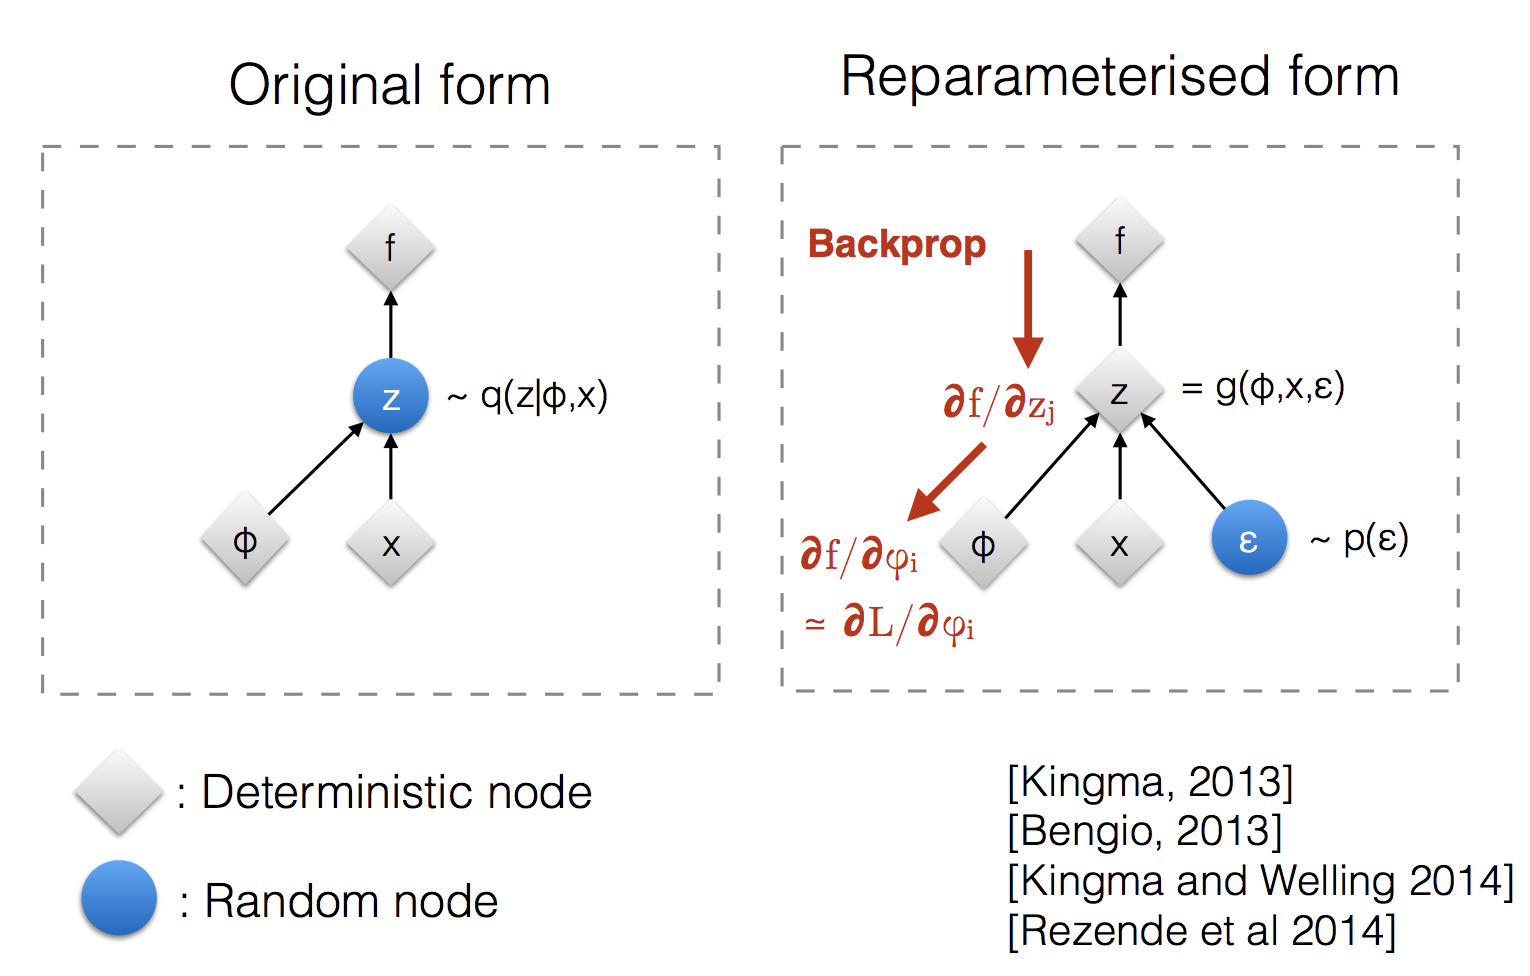
\includegraphics{source/figures/reparameterization-trick.png}

Como ejemplo, una forma común para esto
\(q_{\phi}(\mathbf{z} | \mathbf{x})\) es una Gaussiana multivariable con
estructura de covarianza diagonal.

\[
\begin{array}{l}
\mathbf{z} \sim q_{\phi}\left(\mathbf{z} | \mathbf{x}^{(i)}\right)=\mathcal{N}\left(\mathbf{z} ; \boldsymbol{\mu}^{(i)}, \boldsymbol{\sigma}^{2(i)} \boldsymbol{I}\right) \\
\mathbf{z}=\boldsymbol{\mu}+\boldsymbol{\sigma} \odot \boldsymbol{\epsilon}, \text { where } \boldsymbol{\epsilon} \sim \mathcal{N}(0, \boldsymbol{I})
\end{array}
\]

Donde \(\odot\) corresponde al producto elemento a elemento.

El truco de la reparametrización funciona también para otro tipo de
distribuciones, no solo la Gaussiana. En el caso de la Gaussiana
multivariable, se hace posible entrenar el modelo aprendiendo la media y
la varianza de la distribución. \(\mu\) y \(\sigma\), usando
explícitamente este truco, mientras que la estocásticidad permanece en
la variable aleatoria
\(\boldsymbol{\epsilon} \sim \mathcal{N}(0, \boldsymbol{I})\).

\hypertarget{autoencoders-apilados}{%
\subsection{Autoencoders apilados}\label{autoencoders-apilados}}

Aunque en las secciones anteriores tanto el codificador como el
decodificador se han tratado como dos capas dentro de una red de 3
capas. La realidad es que en muchos casos se necesita más capas tanto a
un lado como a otro. Aquellos autoencoders donde o bien el codificador o
bien el decodificador tienen más de una capa, se les conoce con el
nombre de Autoencoders apilados (\textbf{Stacked Autoencoders}). Al
igual que para el resto de arquitecturas de Deep Learning, añadir más
capas permite reducir la linealidad y aprender patrones más complejos.

El principal factor a tener en cuenta en estos casos, es que los
autoencoders son muy potentes de por si, en relación con la función que
tienen que modelar (identidad). Es por esto, por lo que la
regularización se vuelve esencial a la hora de apilar diferentes capas a
un lado u a otro.

En cuanto a diseño, la forma más común de diseñarlos es de manera
simétrica - el mismo número de capas y unidades para el encoder y el
decoder. Además, las capas suelen tener un número de neuronas
decrecientes para el encoder y crecientes para el decoder. Esto permite
aplicar un técnica conocida como \textbf{Tied Weights}. Esta técnica
consiste en compartir los pesos entre el codificar y el decodificador,
haciendo que los pesos de este último corresponda con la transpuesta del
primero:

\[\theta_{d} = \theta_{e}^T\]

Esta técnica mejor el rendimiento en el entrenamiento, ya que se
entrenan menos parámetros, pero además, sirve como método de
regularización.

\hypertarget{aplicaciones-de-los-autoencoders}{%
\subsection{Aplicaciones de los
autoencoders}\label{aplicaciones-de-los-autoencoders}}

Las aplicaciones principales de los autoencoders han sido la
\textbf{reducción de la dimensionalidad} y \textbf{recuperación de
información}. Autoencoders no lineales pueden ofrecer un error de
reconstrucción menor que PCA, y al no estar limitados a una proyección
lineal, pueden aprender una representación más fácil de interpretar. En
el caso de clasificación, los autoencoders pueden encontrar una
representación donde los datos estén agrupados en clusters y las
categorías estén bien diferenciadas. Además, encontrar una proyección a
un espacio de dimensión inferior que mantenga la mayoría de la
información, permite mejorar el rendimiento de modelos, ya que estos en
espacios inferiores tiene un menor coste de cómputo y memoria.

Otra aplicación que se ha ido desarrollando en los últimos años es la de
\textbf{detección de anomalías}. Los autoencoders pueden utilizarse para
modelar la distribución de datos, y el error de reconstrucción se puede
utilizar como indicador para detectar anomalías. Cuando un autoencoder
se ha entrenado correctamente, el error de reconstrucción sobre datos de
de entrenamiento es bajo. Así como el error otros datos de la misma
distribución que no hayan usado para entrenar (conjunto de validación y
test por ejemplo). Pero en el caso de utilizar datos de una distribución
distinta, al no poder extraer las características más importantes
eficazmente, el error de reconstrucción es mayor. Por este motivo, se
puede entrenar un autoencoder sobre los datos ``no anómalos'', y
establecer un umbral sobre el error de reconstrucción que indique si el
ejemplo que se ha pasado por la red es una anomalía.

Por otro lado, cabe destacar el uso de los autoencoders variacionales
como modelos generativos, aunque se ven opacados en su mayoría por GAN y
similares.

Una última aplicación que cabe destacar es la de \textbf{clasificación}.
Los autoencoders, pese a modelos de aprendizaje no supervisado, pueden
usarse para problemas de clasificación. Si se entrena un autoencoder
para cada clase (con ejemplos exclusivos de esa clase), el error de
reconstrucción de cada autoencoder se puede puede utilizar para decidir
la clase. Presuntamente, aquellos ejemplos cercanos a una determinada
clase, tendrán un error de reconstrucción menor en su autoencoder
correspondiente. De esta forma, podemos aplicar este tipo de
arquitecturas a problemas de clasificación. No obstante, los
autoencoders se entrenan de manera independiente minimizando el error de
reconstrucción y la regularización (si aplica), esto implica que no hay
una optimización directa del error de clasificación. Al perder esa
relación directa con la métrica objetiva, este aplicación puede dar
lugar a resultados subóptimos.

\hypertarget{estado-del-arte}{%
\section{Estado del Arte}\label{estado-del-arte}}

\hypertarget{planificaciuxf3n-del-trabajo}{%
\chapter{Planificación del trabajo}\label{planificaciuxf3n-del-trabajo}}

\begin{itemize}
\tightlist
\item
  Planificación optimista
\item
  Planificación real
\end{itemize}

\hypertarget{presupuesto}{%
\chapter{Presupuesto}\label{presupuesto}}

\begin{itemize}
\tightlist
\item
  Comparitiva cluster propio vs AWS, Azure, GDC
\item
  Coste de titulado superior (36€)
\end{itemize}

\hypertarget{diseuxf1o-del-marco-de-trabajo}{%
\chapter{Diseño del marco de
trabajo}\label{diseuxf1o-del-marco-de-trabajo}}

\hypertarget{herramientas-utilizadas}{%
\section{Herramientas utilizadas}\label{herramientas-utilizadas}}

\hypertarget{estructura-general}{%
\section{Estructura general}\label{estructura-general}}

\hypertarget{tracking-de-experimentos}{%
\section{Tracking de experimentos}\label{tracking-de-experimentos}}

\hypertarget{hiperparametrizaciuxf3n-y-entrenamiento-distribuido}{%
\section{Hiperparametrización y entrenamiento
distribuido}\label{hiperparametrizaciuxf3n-y-entrenamiento-distribuido}}

\hypertarget{sistema-de-notificaciones-y-callbacks}{%
\section{Sistema de notificaciones y
callbacks}\label{sistema-de-notificaciones-y-callbacks}}

\hypertarget{interfaz-web}{%
\section{Interfaz Web}\label{interfaz-web}}

\hypertarget{otras-herramientas-para-la-reproducibilidad}{%
\section{Otras herramientas para la
reproducibilidad}\label{otras-herramientas-para-la-reproducibilidad}}

\hypertarget{futuro-desarrollo}{%
\section{Futuro desarrollo}\label{futuro-desarrollo}}

\hypertarget{experimentos}{%
\chapter{Experimentos}\label{experimentos}}

\hypertarget{diseuxf1o-del-autoencoder}{%
\section{Diseño del autoencoder}\label{diseuxf1o-del-autoencoder}}

\begin{itemize}
\tightlist
\item
  Autoencoder simple
\item
  Autoencoder profundo
\item
  Autoencoder variacional
\end{itemize}

\hypertarget{resultados}{%
\section{Resultados}\label{resultados}}

\hypertarget{anexo-manual-de-usuario}{%
\chapter{Anexo: Manual de Usuario}\label{anexo-manual-de-usuario}}

\footnotesize

\hypertarget{referencias}{%
\chapter{Referencias}\label{referencias}}

\end{document}
